\documentclass{article}

% Language setting
% Replace `english' with e.g. `spanish' to change the document language
\usepackage{biblatex} %Imports biblatex package
\addbibresource{refs.bib}
\usepackage[english]{babel}
\usepackage{array}
\usepackage{amsmath}
\usepackage{pythonhighlight}
\usepackage{multirow}
\newcolumntype{P}[1]{>{\centering\arraybackslash}p{#1}}
\newcolumntype{M}[1]{>{\centering\arraybackslash}m{#1}}

% Set page size and margins
% Replace `letterpaper' with `a4paper' for UK/EU standard size
\usepackage[letterpaper,top=2cm,bottom=2cm,left=3cm,right=3cm,marginparwidth=1.75cm]{geometry}

\usepackage{amsmath}
\usepackage{graphicx}
\usepackage[colorlinks=true, allcolors=blue]{hyperref}
\usepackage{setspace}
\usepackage{booktabs}
\usepackage[T1]{fontenc}
\usepackage{longtable}
\doublespacing

\begin{document}
\begin{titlepage}

\centering
\scshape
\vspace{\baselineskip}

%
\rule{\textwidth}{1.6pt}\vspace*{-\baselineskip}\vspace*{2pt}
\rule{\textwidth}{0.4pt}

{\Huge \textbf{\textsc{ Tensile Stress-Strain \\
\vspace{15pt}}}}

\rule{\textwidth}{0.4pt}\vspace*{-\baselineskip}\vspace{3.2pt}
\rule{\textwidth}{1.6pt}\vspace{6pt}
\centerline{\textit{University of Illinois at Urbana-Champaign}} 
\centerline{\textit{Department of Nuclear, Plasma, and Radiological Engineering}}
\vspace{1.5\baselineskip}


\large \centerline{\textbf{Author:} Nathan Glaser}
\large \centerline{\textbf{Net-ID:} nglaser3}
\quad

\vfill
\large \centerline{September 25, 2024}
%
\pagenumbering{gobble}
\end{titlepage}

\tableofcontents
\newpage
\pagenumbering{arabic}

\section{Abstract}

\newpage
\section{Introduction}
An exceedingly common loading condition to test for engineering materials strength and deformation properties is uniaxially. An example of this type of loading condition is a tension or compression test, in which the specimen is loaded and either pulled / compressed until failure or the desired outcome fruitions. These tests measure the stress, the axial force applied to the specimen, and the strain, the dimensional change the specimen undergoes due to loading.
\subsection{Stress and Strain}
Tension and compression tests both load and measure axially, and thus do not take into consideration non-1D changes in geometry. Thus, these tests yield what is commonly named 'engineering' stress/strain. To determine the engineering stress/strain is very simple. The strain is simply how much the specimen is compressed due to the load and is directly measured by the testing apparatus. The stress is simply the force applied by the testing apparatus divided by the cross sectional area of the point of interest on the specimen. 
\begin{equation}
    \sigma_e = \frac{F}{A_o}
    \label{eq:engstress}
\end{equation}

Next, to adjust engineering stress/strain to closer represent the stress and strain the point of interest in the specimen actually undergoes, we utilize Eqs. \ref{eq:trustress} and \ref{eq:trustrain} to convert to true stress/strain.

\begin{equation}
    \sigma_t = \sigma_e \left(1+ \epsilon_e \right)
    \label{eq:trustress}
\end{equation}
\begin{equation}
    \epsilon_t = ln\left(1+\epsilon_e\right)
    \label{eq:trustrain}
\end{equation}

\subsection{Elastic and Plastic Deformation}
Materials undergo two types of macroscopic deformation: Elastic and Plastic. Elastic deformation is characterized as deformation that the material can 'spring' back from, or recover from, and revert to its initial geometry prior to the most recent loading phase. Elastic deformation, as visualized on an engineering stress/strain plot, is the region in which the stress is linearly related to the strain, with the slope of this region being the Young's modulus (elastic modulus or E are common pseudonyms). The general equation for elastic modulus is Eq. \ref{eq:elasmod}. 
\begin{equation}
    \sigma = E\epsilon
    \label{eq:elasmod}
\end{equation}

Plastic deformation is characterized as deformation that the material cannot recover from. In this region, the relationship between stress and strain is more complicated, but is typically approximated using Eq. \ref{eq:powlaw}, the power law model.
\begin{equation}
    \sigma = K \left( \epsilon\right)^n
    \label{eq:powlaw}
\end{equation}

\subsection{Strength and Hardness}
Various metrics are utilized to quantify the strength and hardness of a material. First, to quantify strength a common metric is the 0.2\% Offset Yield Strength (henceforth simplified to Yield Strength) in which a line with slope equalling the elastic modulus and an x-intercept at 0.2\% strain is used. The intersection point of the linear line and the stress-strain curve is the Yield Strength. Further, the Ultimate Tensile Strength (henceforth UTS) is simply the maximum engineering stress the specimen endures. Next, various quantities are utilized to measure a material's hardness. Various tests are utilized: Rockwell A/B/C, Brinnel, Vickers, and more. These utilize an indenter, and forcibly indent a material. The residual indentation is measured and inserted into respective equations to yield hardness values. Another means to quantify a material's hardness is through the modulus of resilience, found utilizing Eq. \ref{eq:modresil}:

\begin{equation}
    U_r = \frac{\left(\sigma_y\right)^2}{2E} 
    \label{eq:modresil}
\end{equation}

where $\sigma_y$ and $E$ are the Yield Strength and Elastic Modulus, respectively. 

\section{Experimental Methods}

\newpage
\section{Results}

\subsection{Question 1}
To begin, we measured the axial load and engineering strain of 6 materials: 
\begin{figure}[!h!]
    \centering
    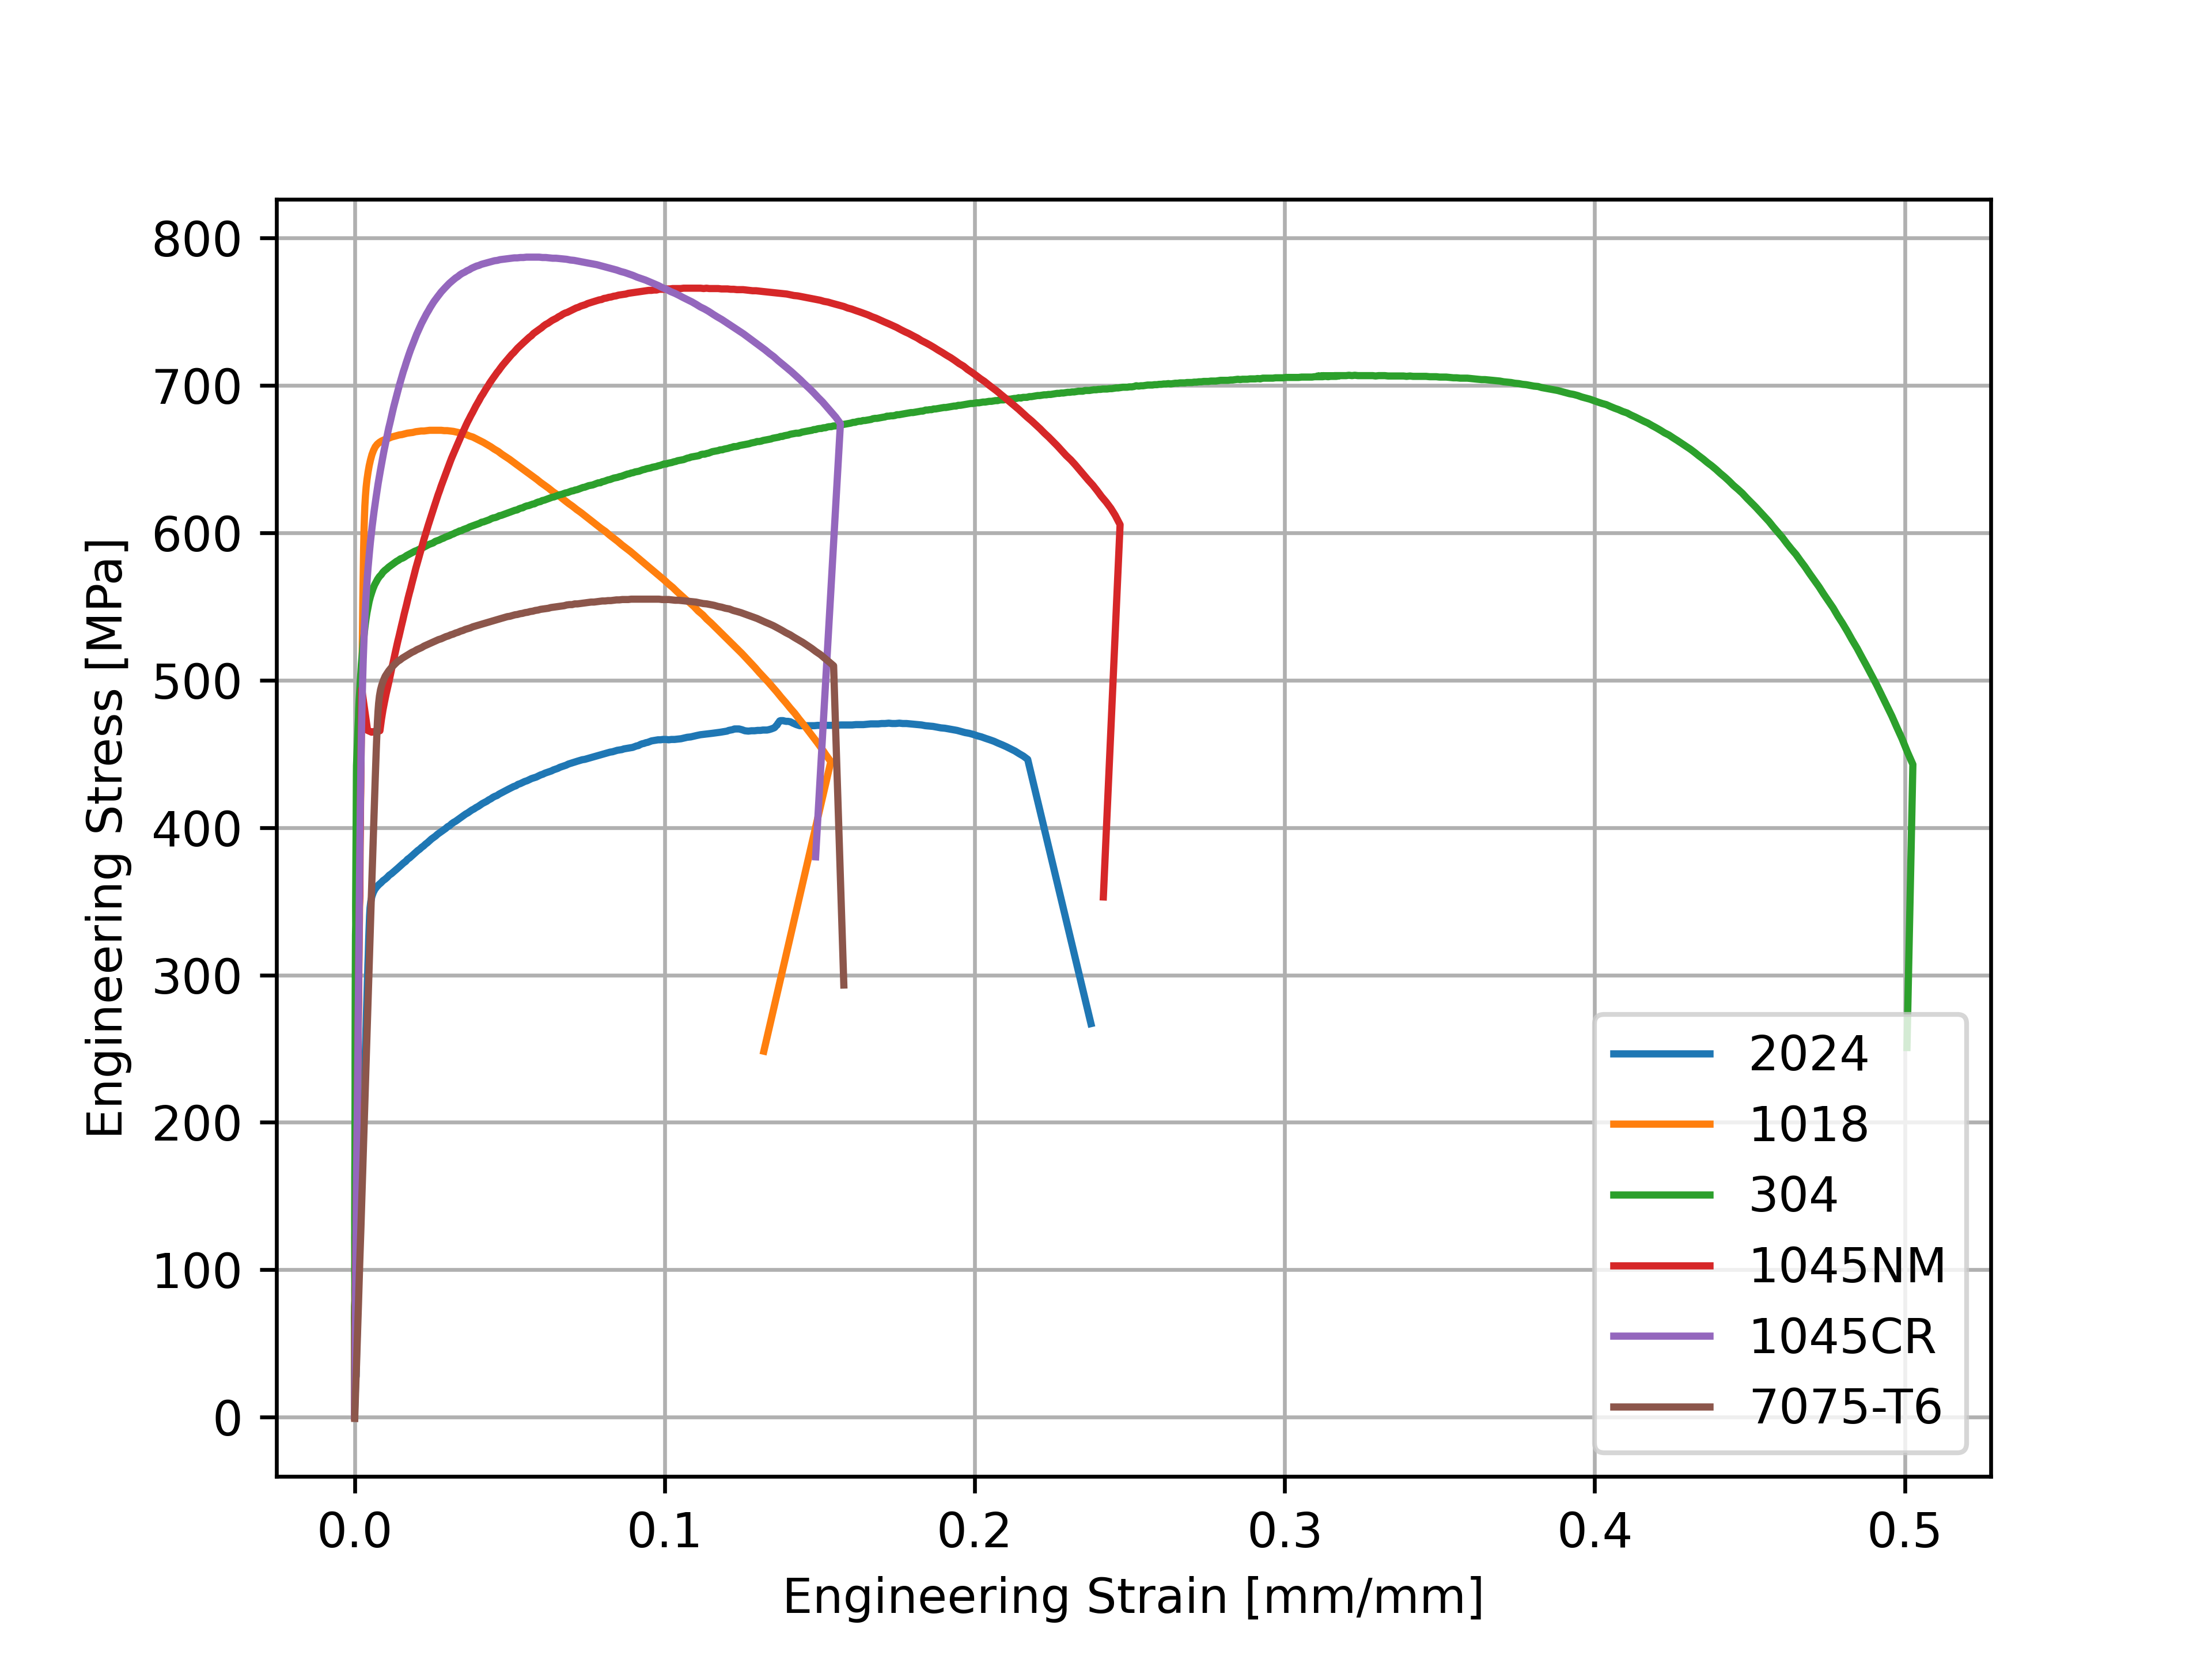
\includegraphics[width=0.5\linewidth]{plots/q1all.png}
    \caption{Caption}
    \label{fig:q1all}
\end{figure}

\begin{figure}[!h!]
    \centering
    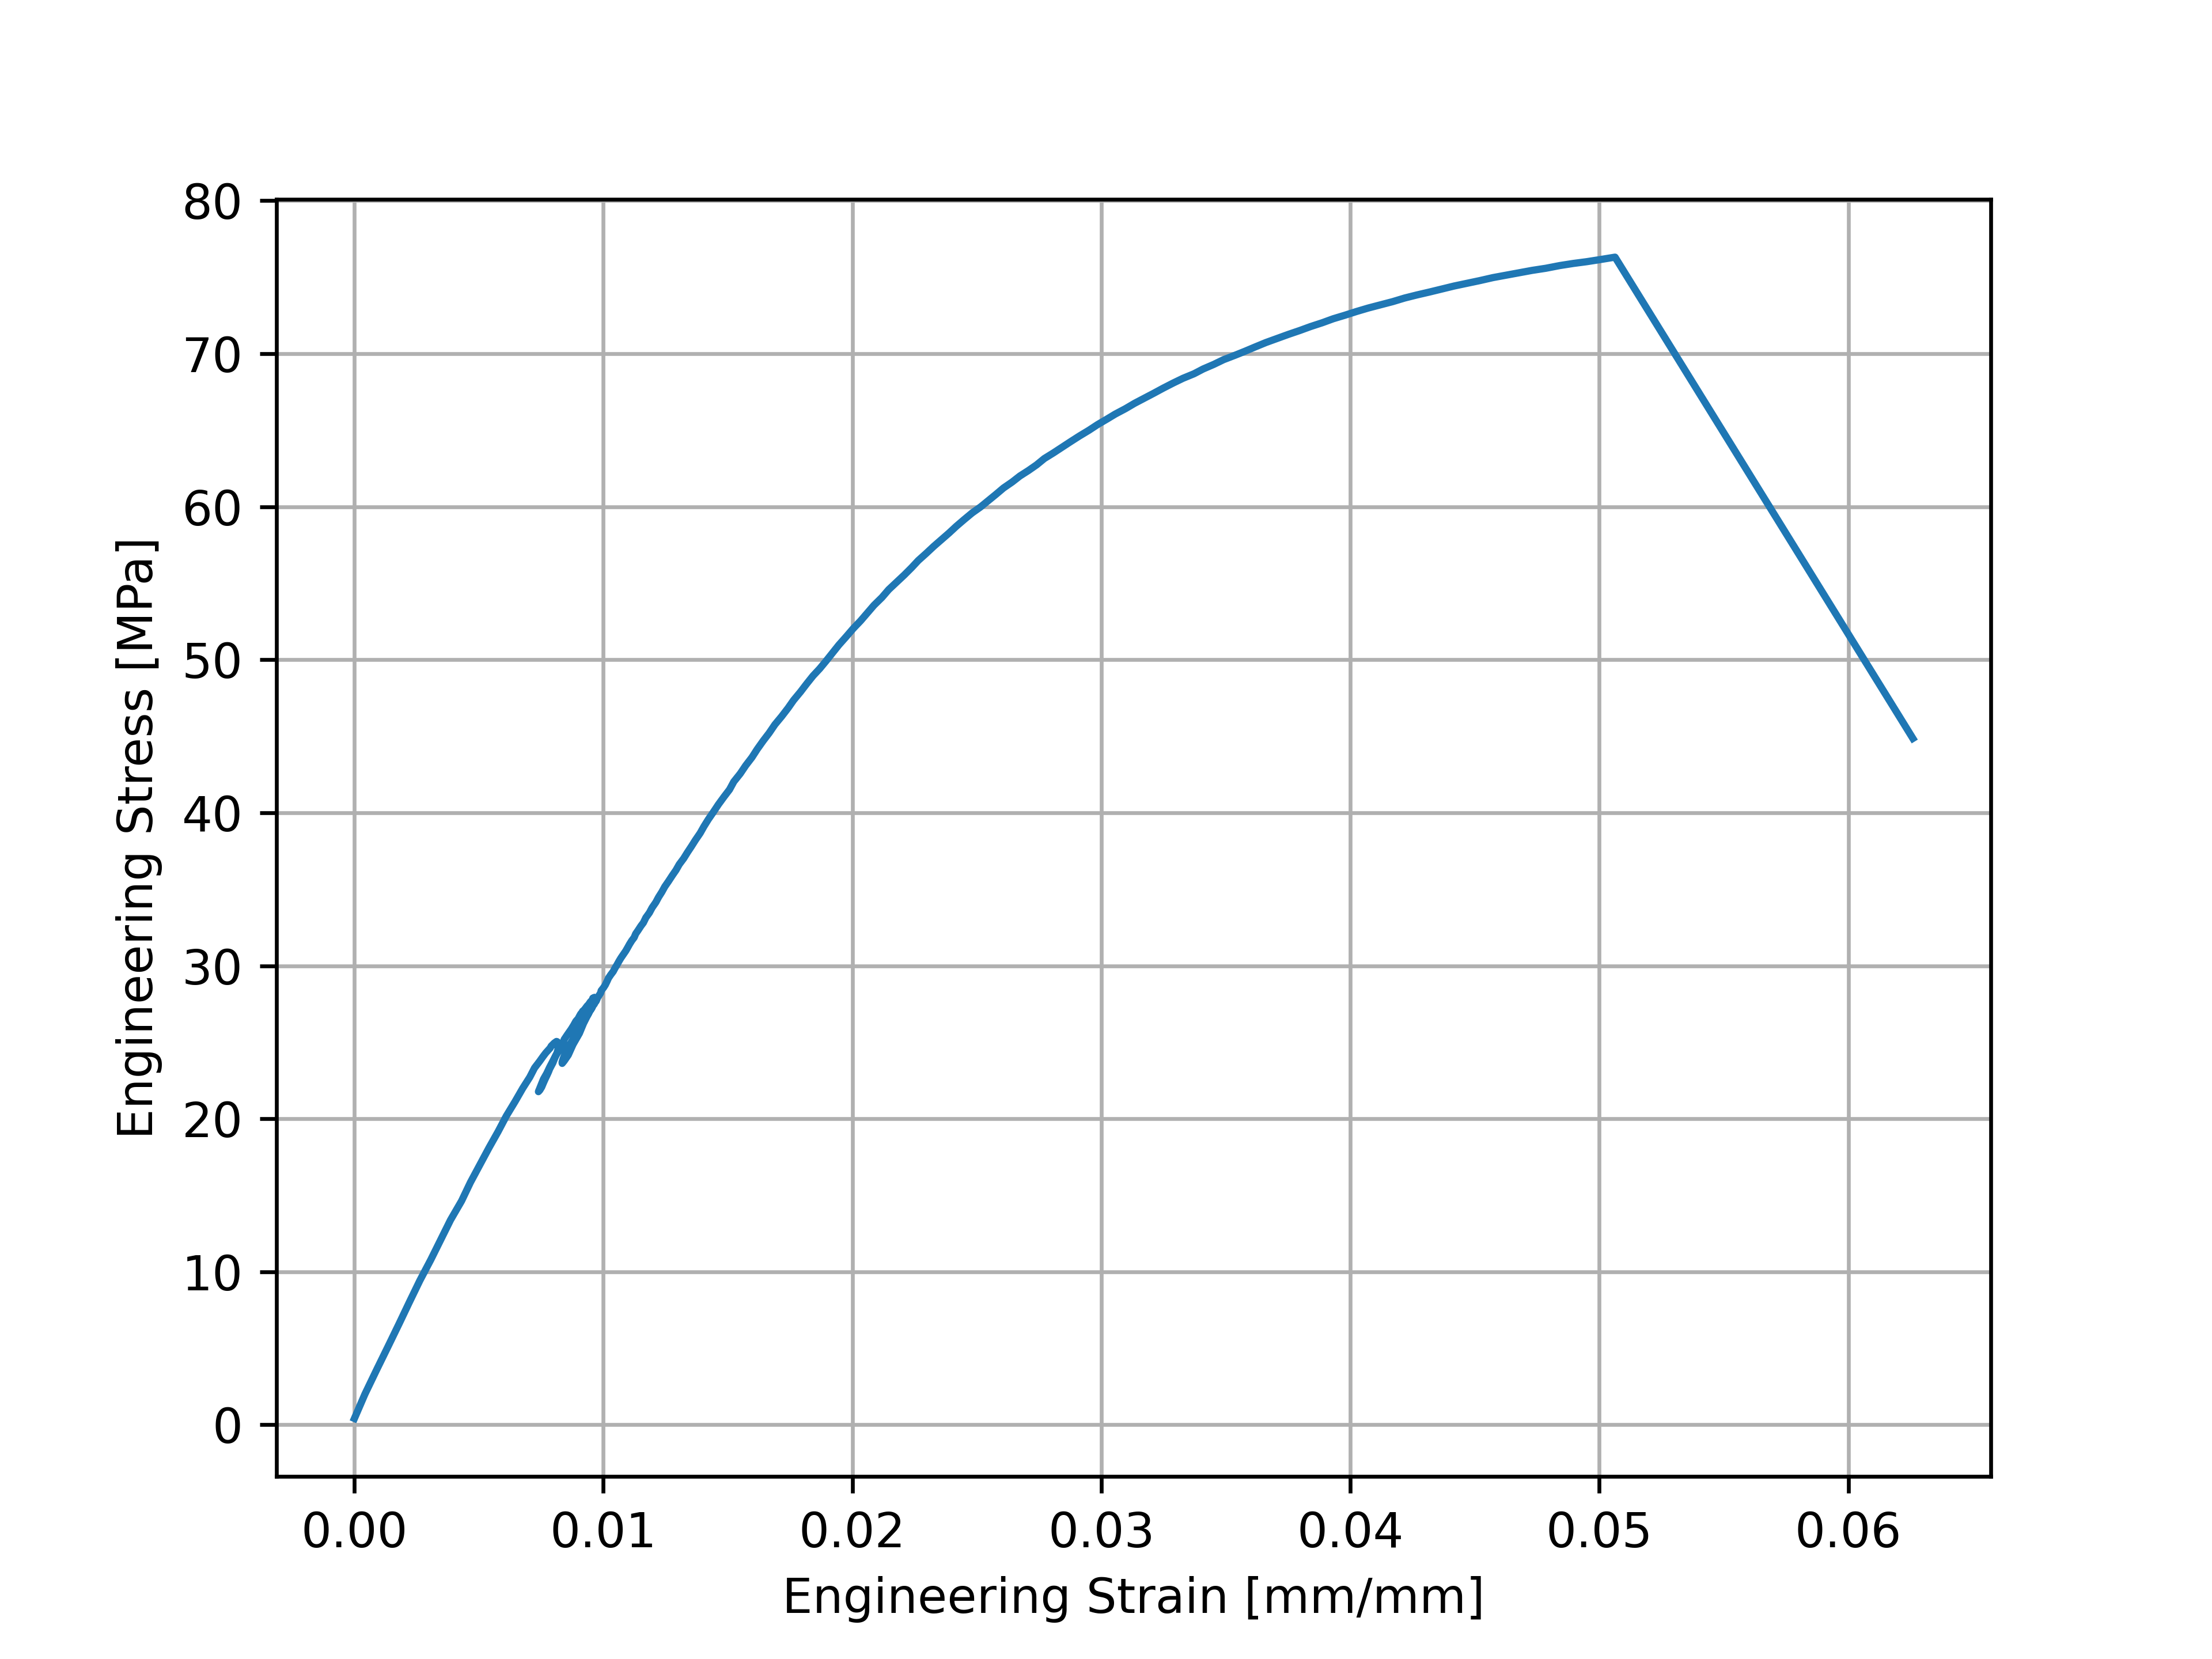
\includegraphics[width=0.5\linewidth]{plots/q1_PMMA.png}
    \caption{Caption}
    \label{fig:q1pmma}
\end{figure}

\subsection{Question 2}

\begin{table}[!h!]
    \centering
    \def\arraystretch{1.5}
    \caption{Tensile material properties for selected materials.}
    \begin{tabular}{|c|c|c|c|c|c|c|c|}
         \toprule
         \hline
         \textbf{Material}& \textbf{2024} & \textbf{PMMA} & \textbf{1018CR} & \textbf{304} & \textbf{1045CR} &\textbf{1045NM} & \textbf{304SS}\\
         \midrule
         \hline
         \textbf{Elastic Modulus [GPa]}& 71.8 & 3.15 & 204.34 & 670.38 & 203.45 & 220.62 & 66.14 \\
         \textbf{Yield Strength [MPa]} & 359.4 & 42.7 & 649.8 & 525.3 & 465.8 & 583.4 & 501.2 \\
         \textbf{UTS [MPa]} & 472.55 & 76.31 & 669.53 & 706.86 & 765.95 & 787.01 & 554.96 \\
         \textbf{\% Elongated} & 23.75 & 6.26 & 15.36 & 50.26 & 24.69 & 15.67 & 15.77 \\
         \textbf{Mod. of Res.} & 0.9 & 0.29 & 1.03 & 0.21 & 0.53 & 0.77 & 1.9\\
         \textbf{R\textsubscript{B} Hardness} & 72.8 & N/A & 94.3 & 100.6 & 90.7 & 96.1 & 86.8 \\
         \hline
    \end{tabular}
    \label{tab:q2}
\end{table}


\newpage
\subsection{Question 3}

\begin{figure}[!h!] 
  \label{fig:q3} 
  \begin{minipage}[b]{0.5\linewidth}
    \centering
    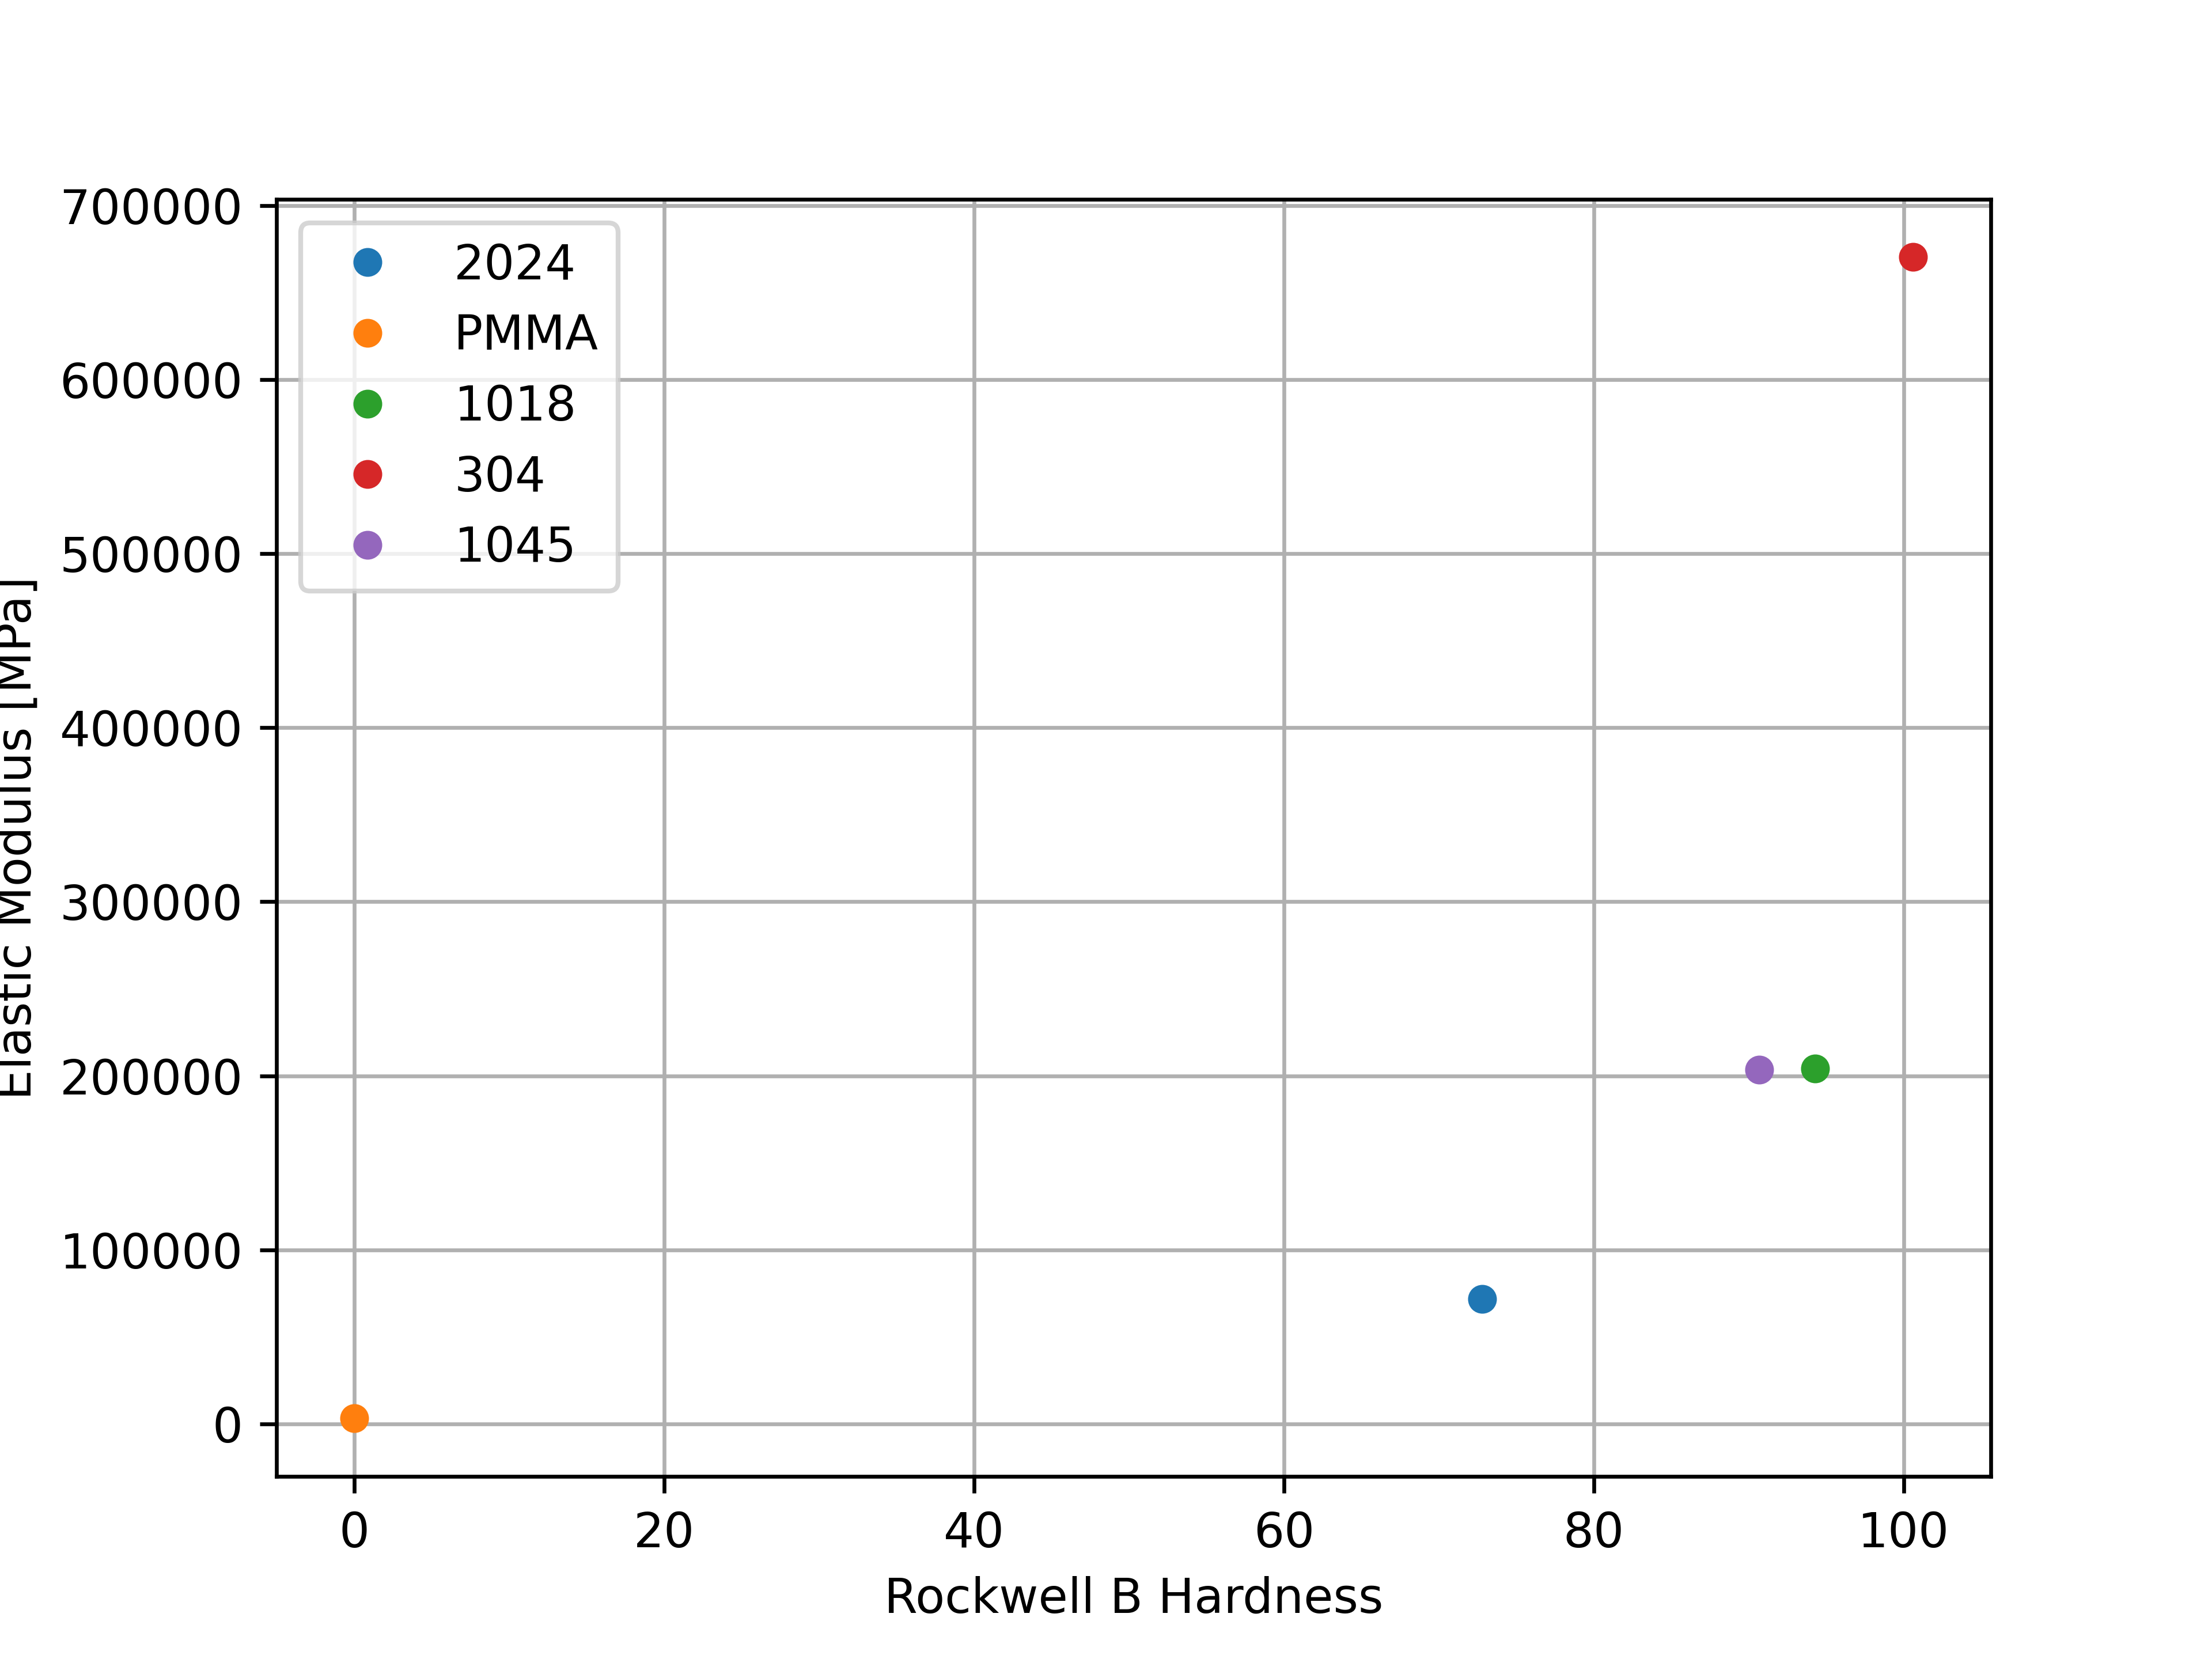
\includegraphics[width=\linewidth]{plots/q3_E.png} 
    \caption{Elastic Modulus as a function \\  of material hardness} 
    \vspace{4ex}
  \end{minipage}
  \begin{minipage}[b]{0.5\linewidth}
    \centering
    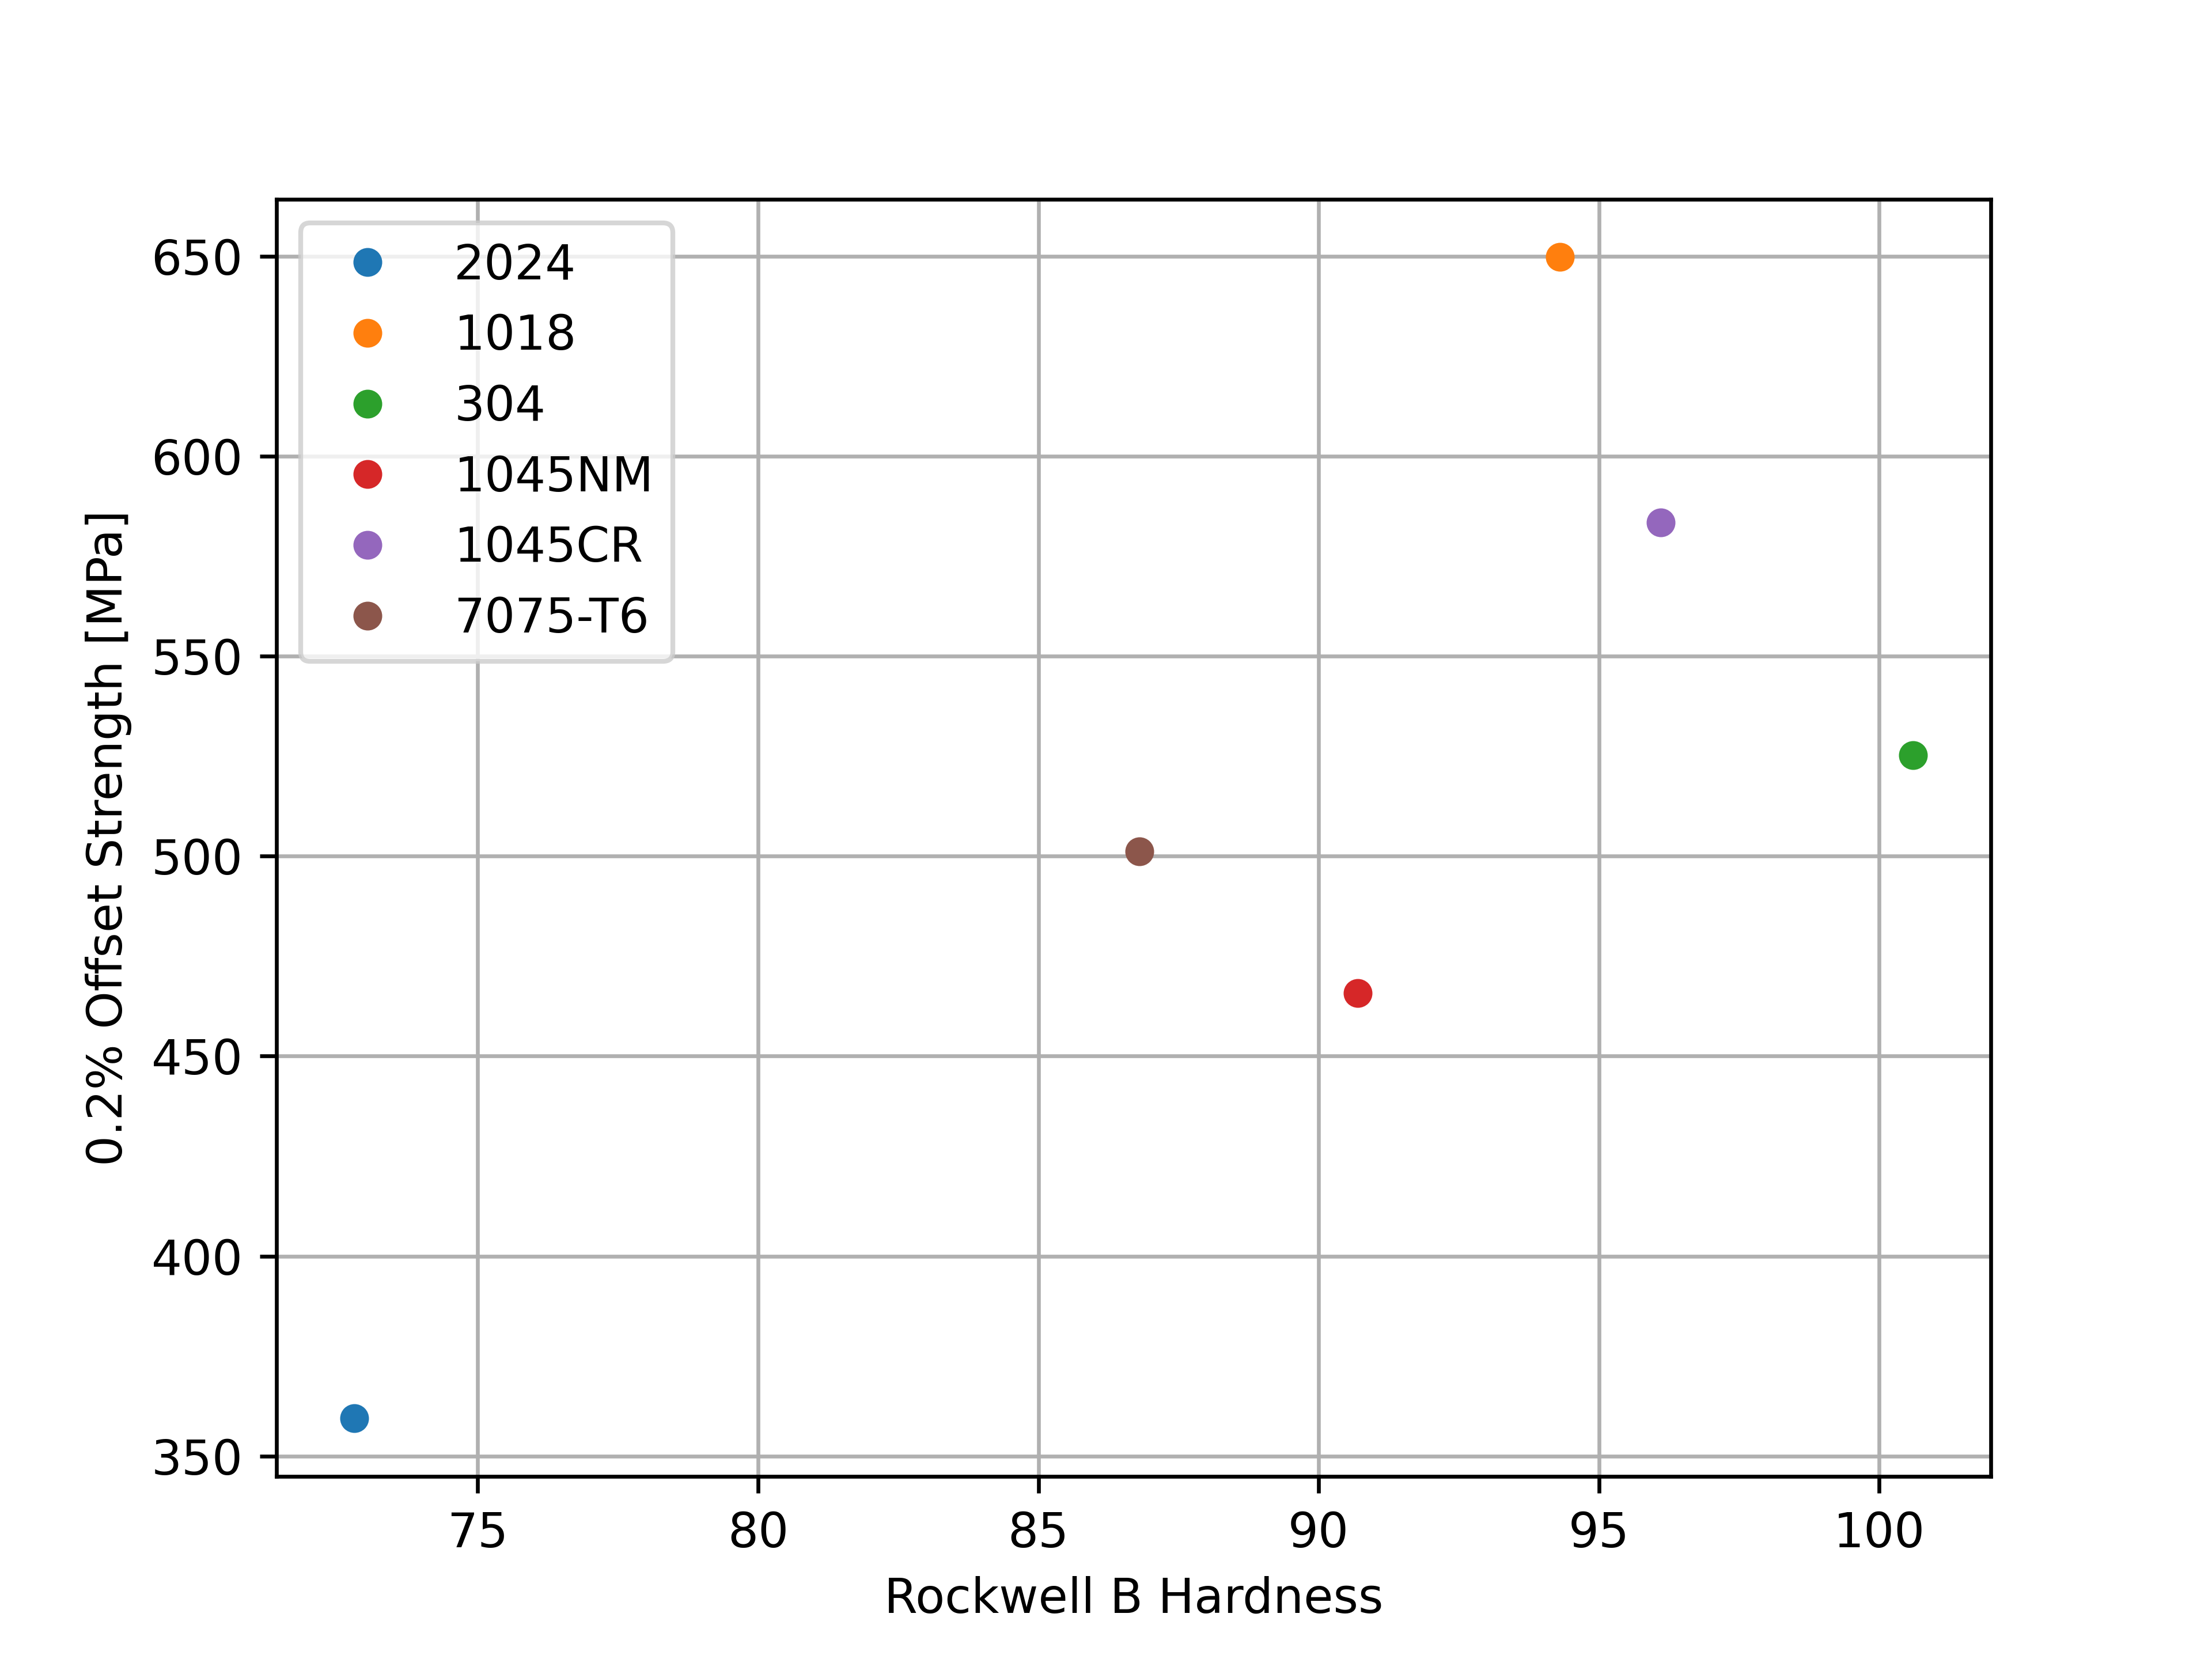
\includegraphics[width=\linewidth]{plots/q3_offstr.png} 
    \caption{Yield Strength as a function \\ of material hardness} 
    \vspace{4ex}
  \end{minipage} 
  \begin{minipage}[b]{0.5\linewidth}
    \centering
    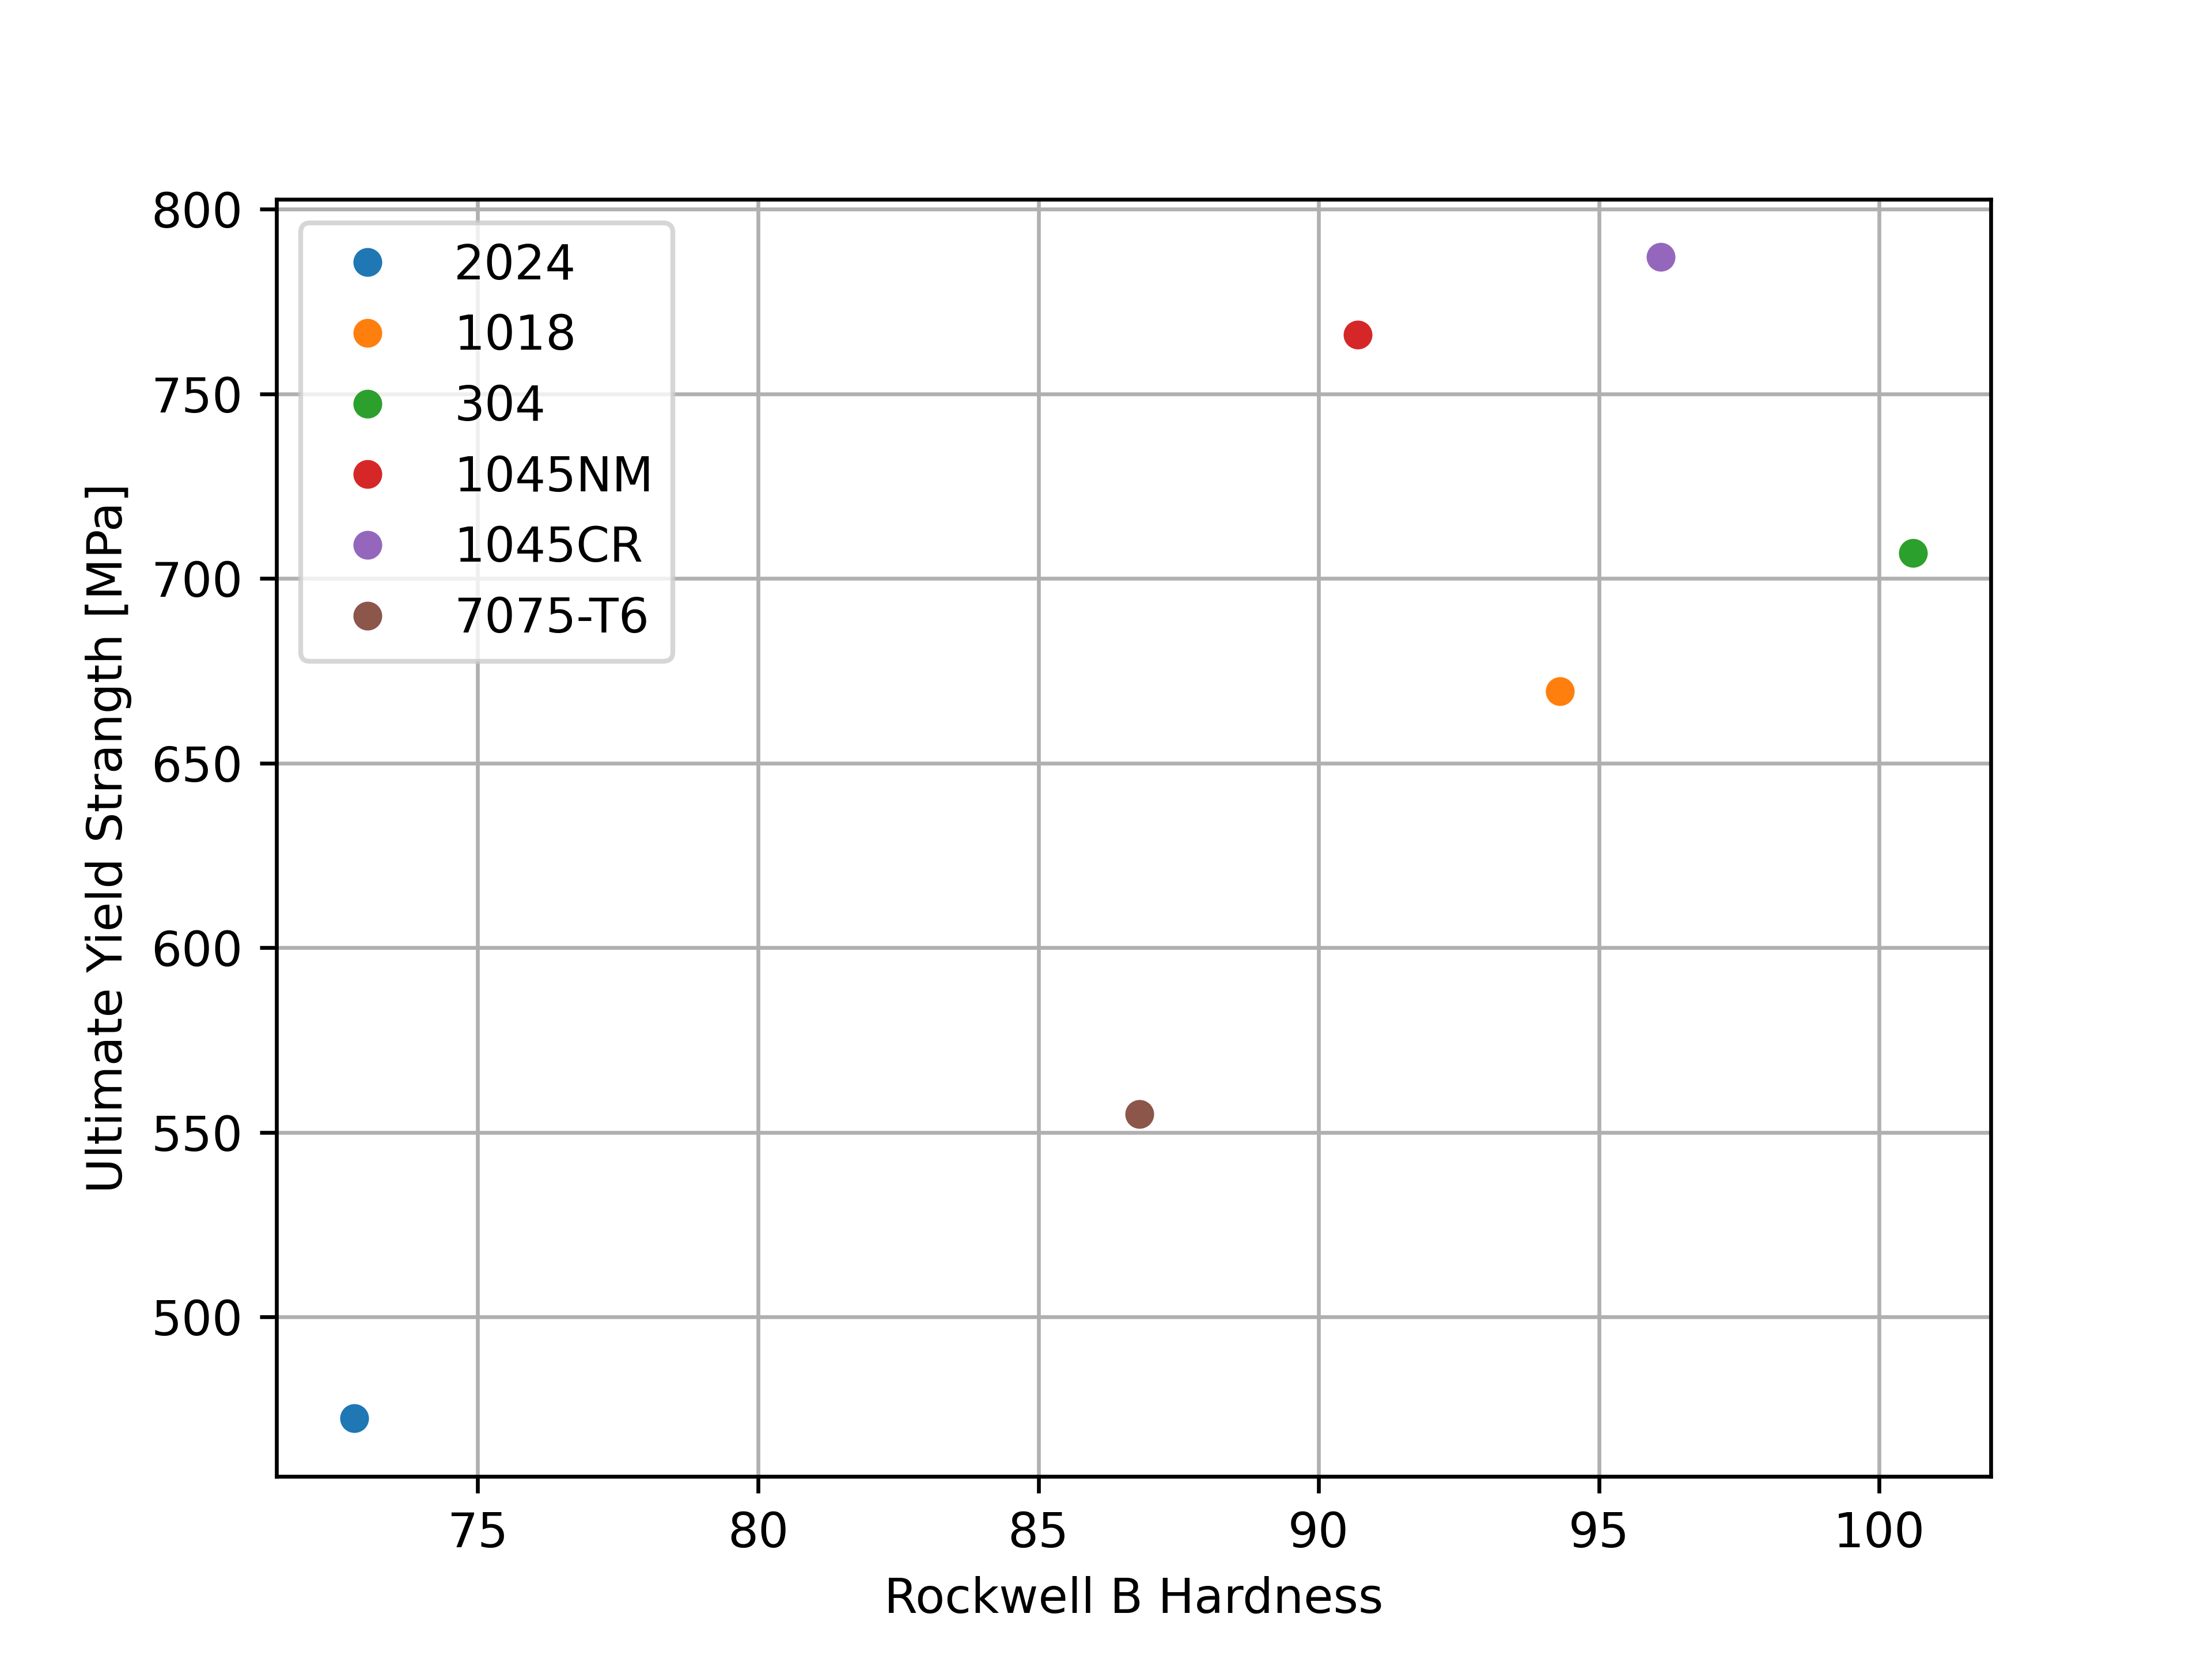
\includegraphics[width=\linewidth]{plots/q3_uts.png} 
    \caption{Ultimate Tensile Strength as a \\ function of material hardness} 
    \vspace{4ex}
  \end{minipage}
  \begin{minipage}[b]{0.5\linewidth}
    \centering
    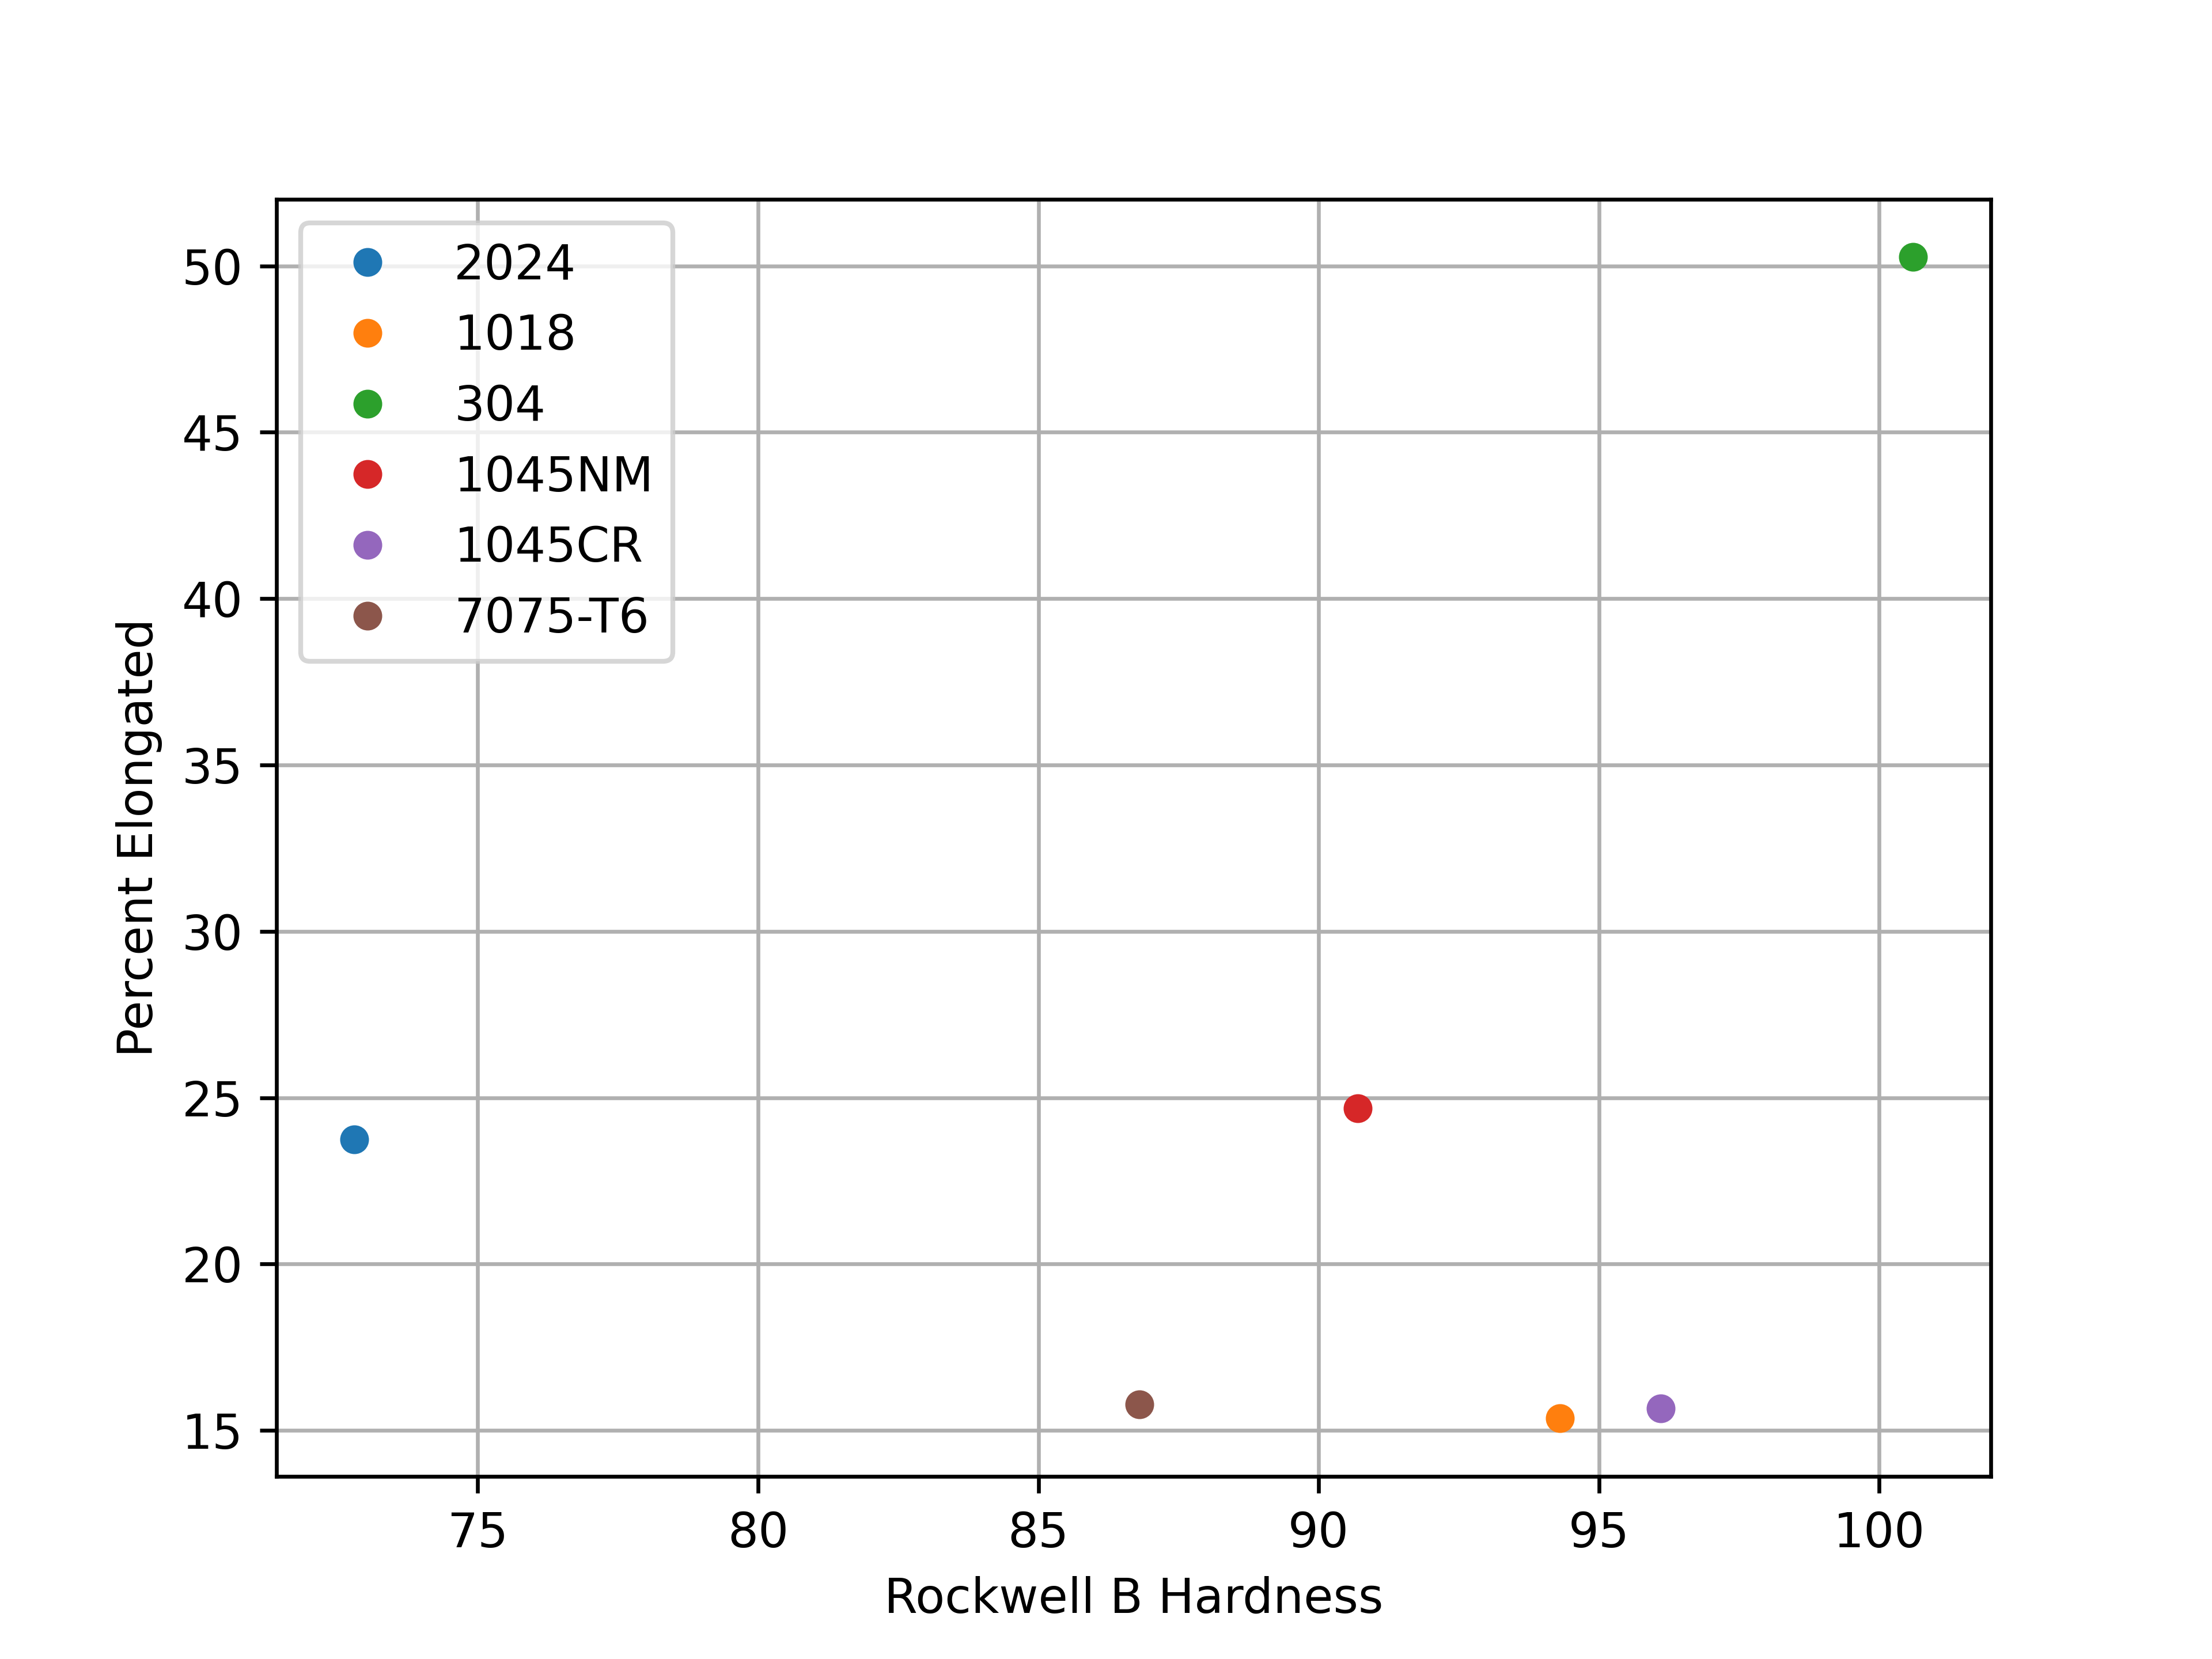
\includegraphics[width=\linewidth]{plots/q3_perelong.png} 
    \caption{Percent Elongation as a function \\ of material hardness} 
    \vspace{4ex}
  \end{minipage} 
  \begin{minipage}[b]{\linewidth}
      \centering
      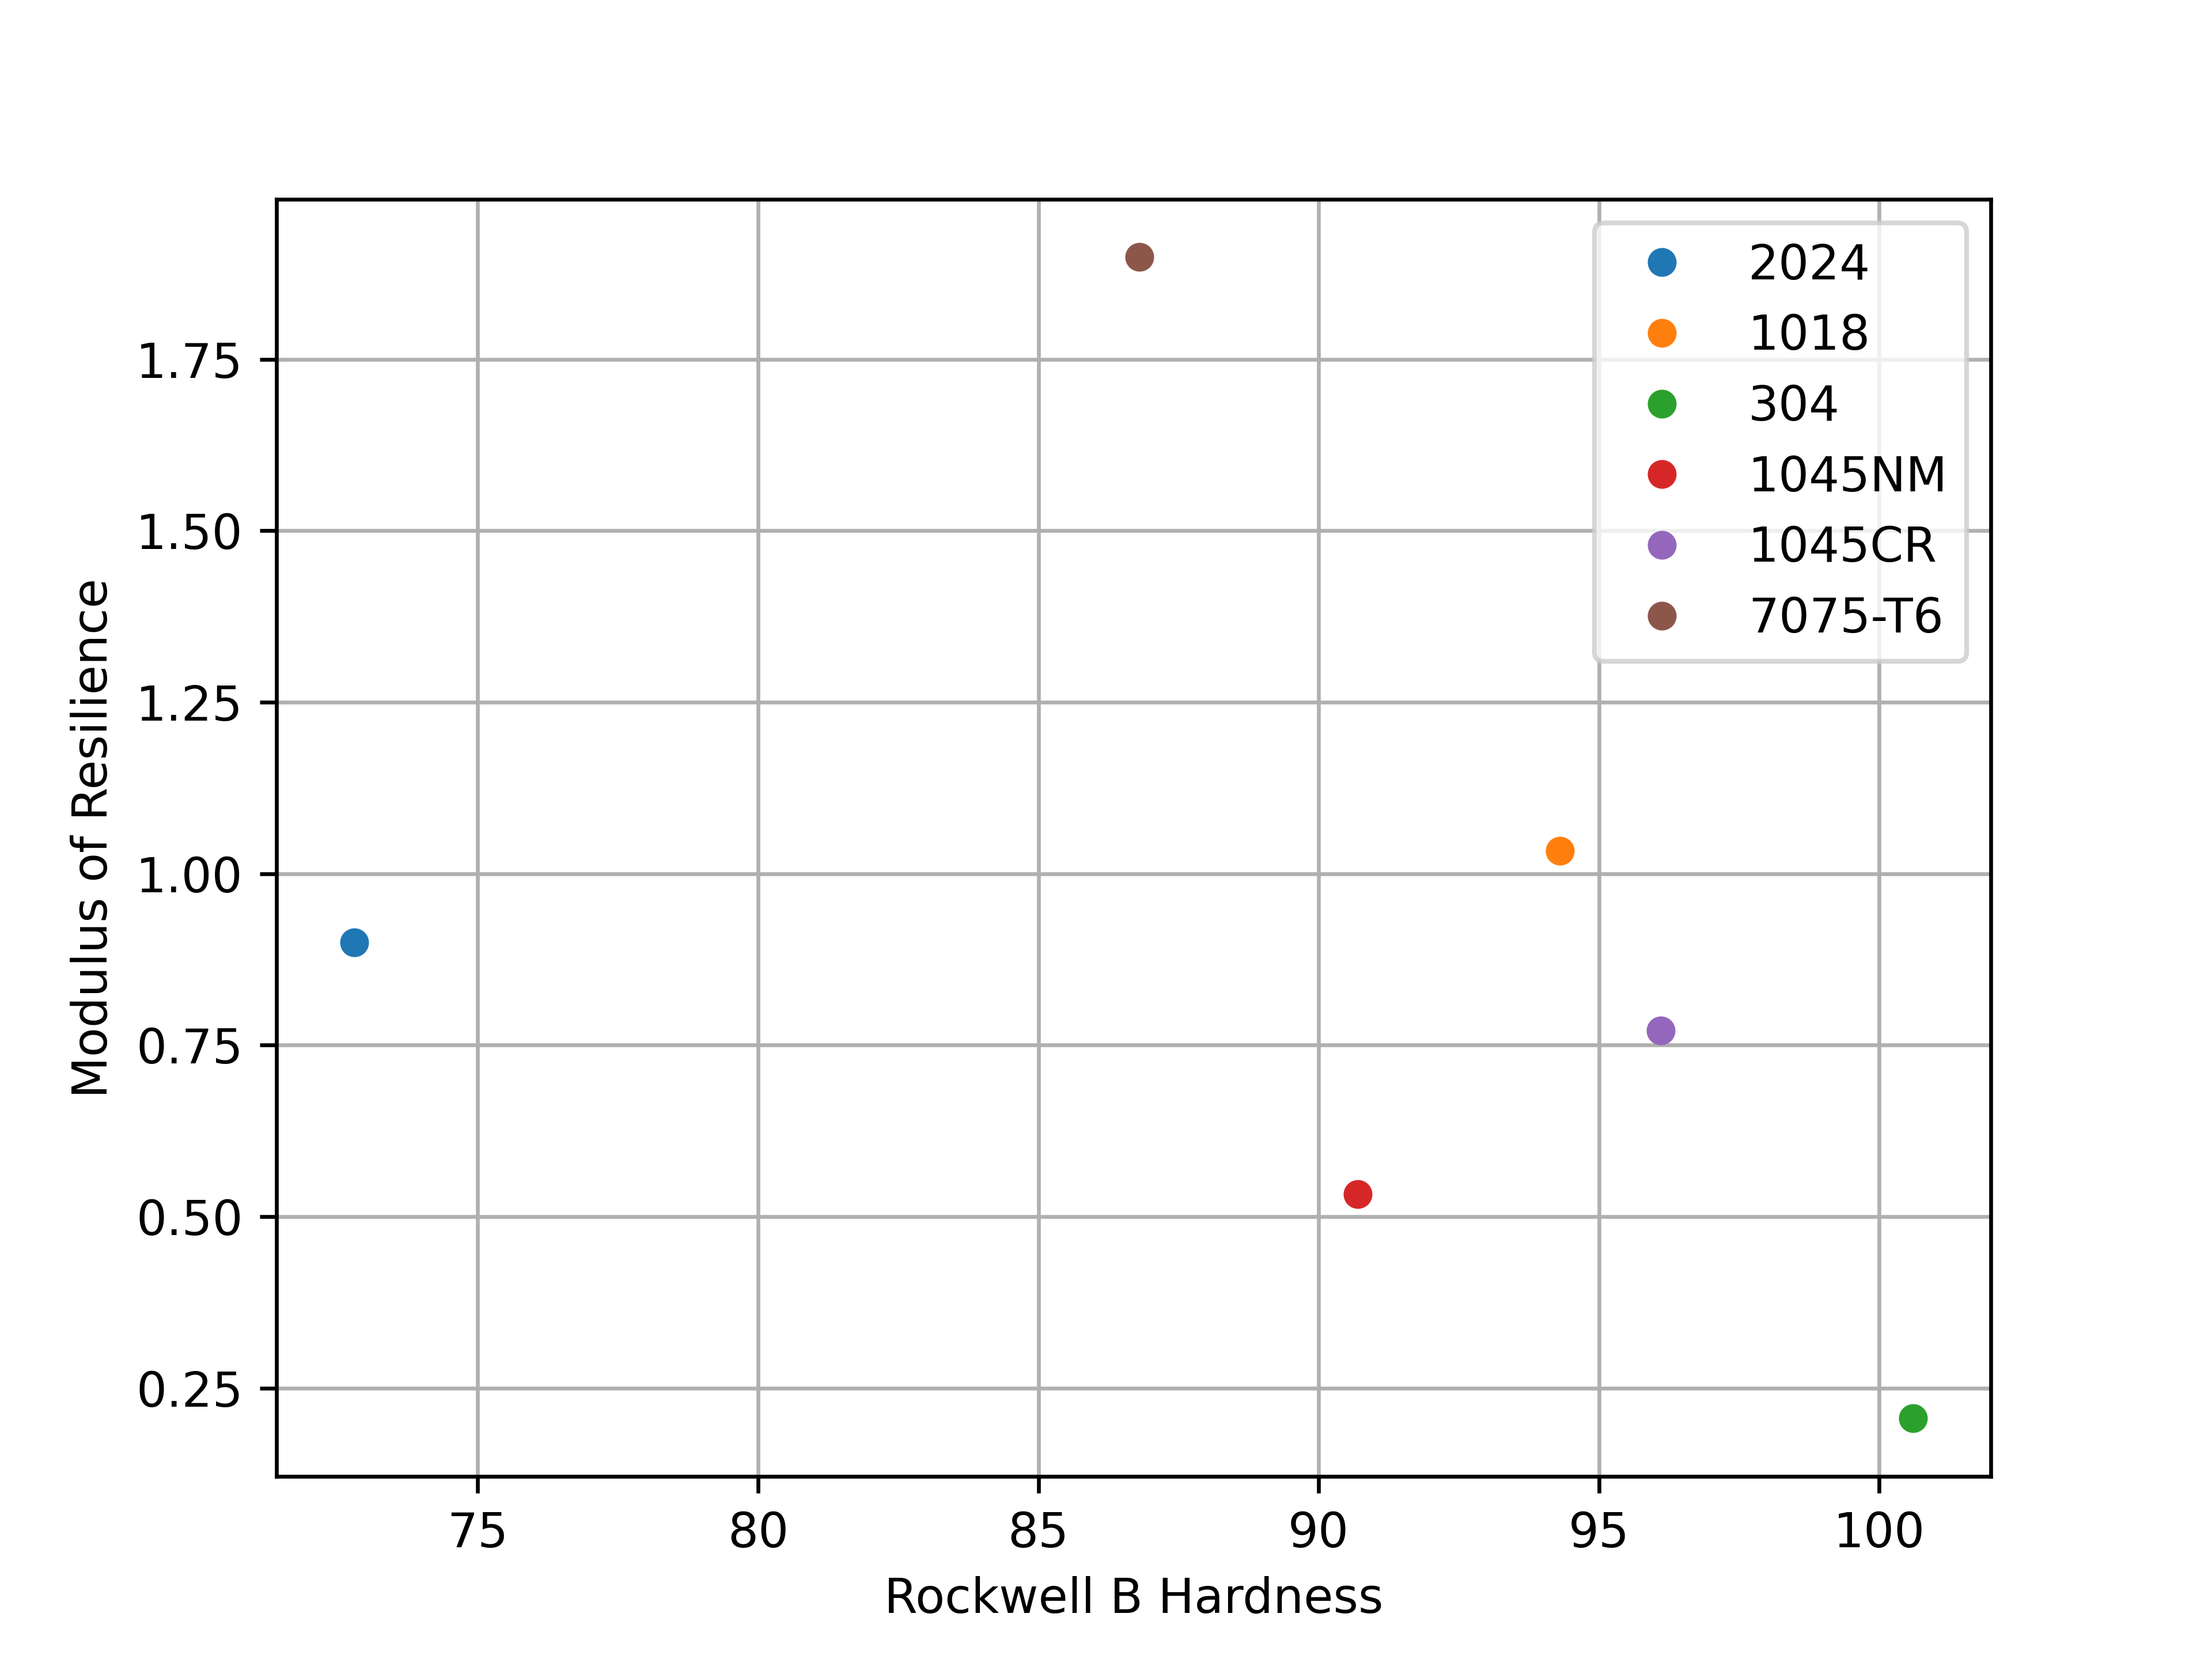
\includegraphics[width = .5\linewidth]{plots/q3_resilmod.png}
      \caption{Modulus of Resilience as a function of material hardness}
  \end{minipage}
\end{figure}
\newpage

\subsection{Question 4}
\begin{figure}[!h]
    \centering
    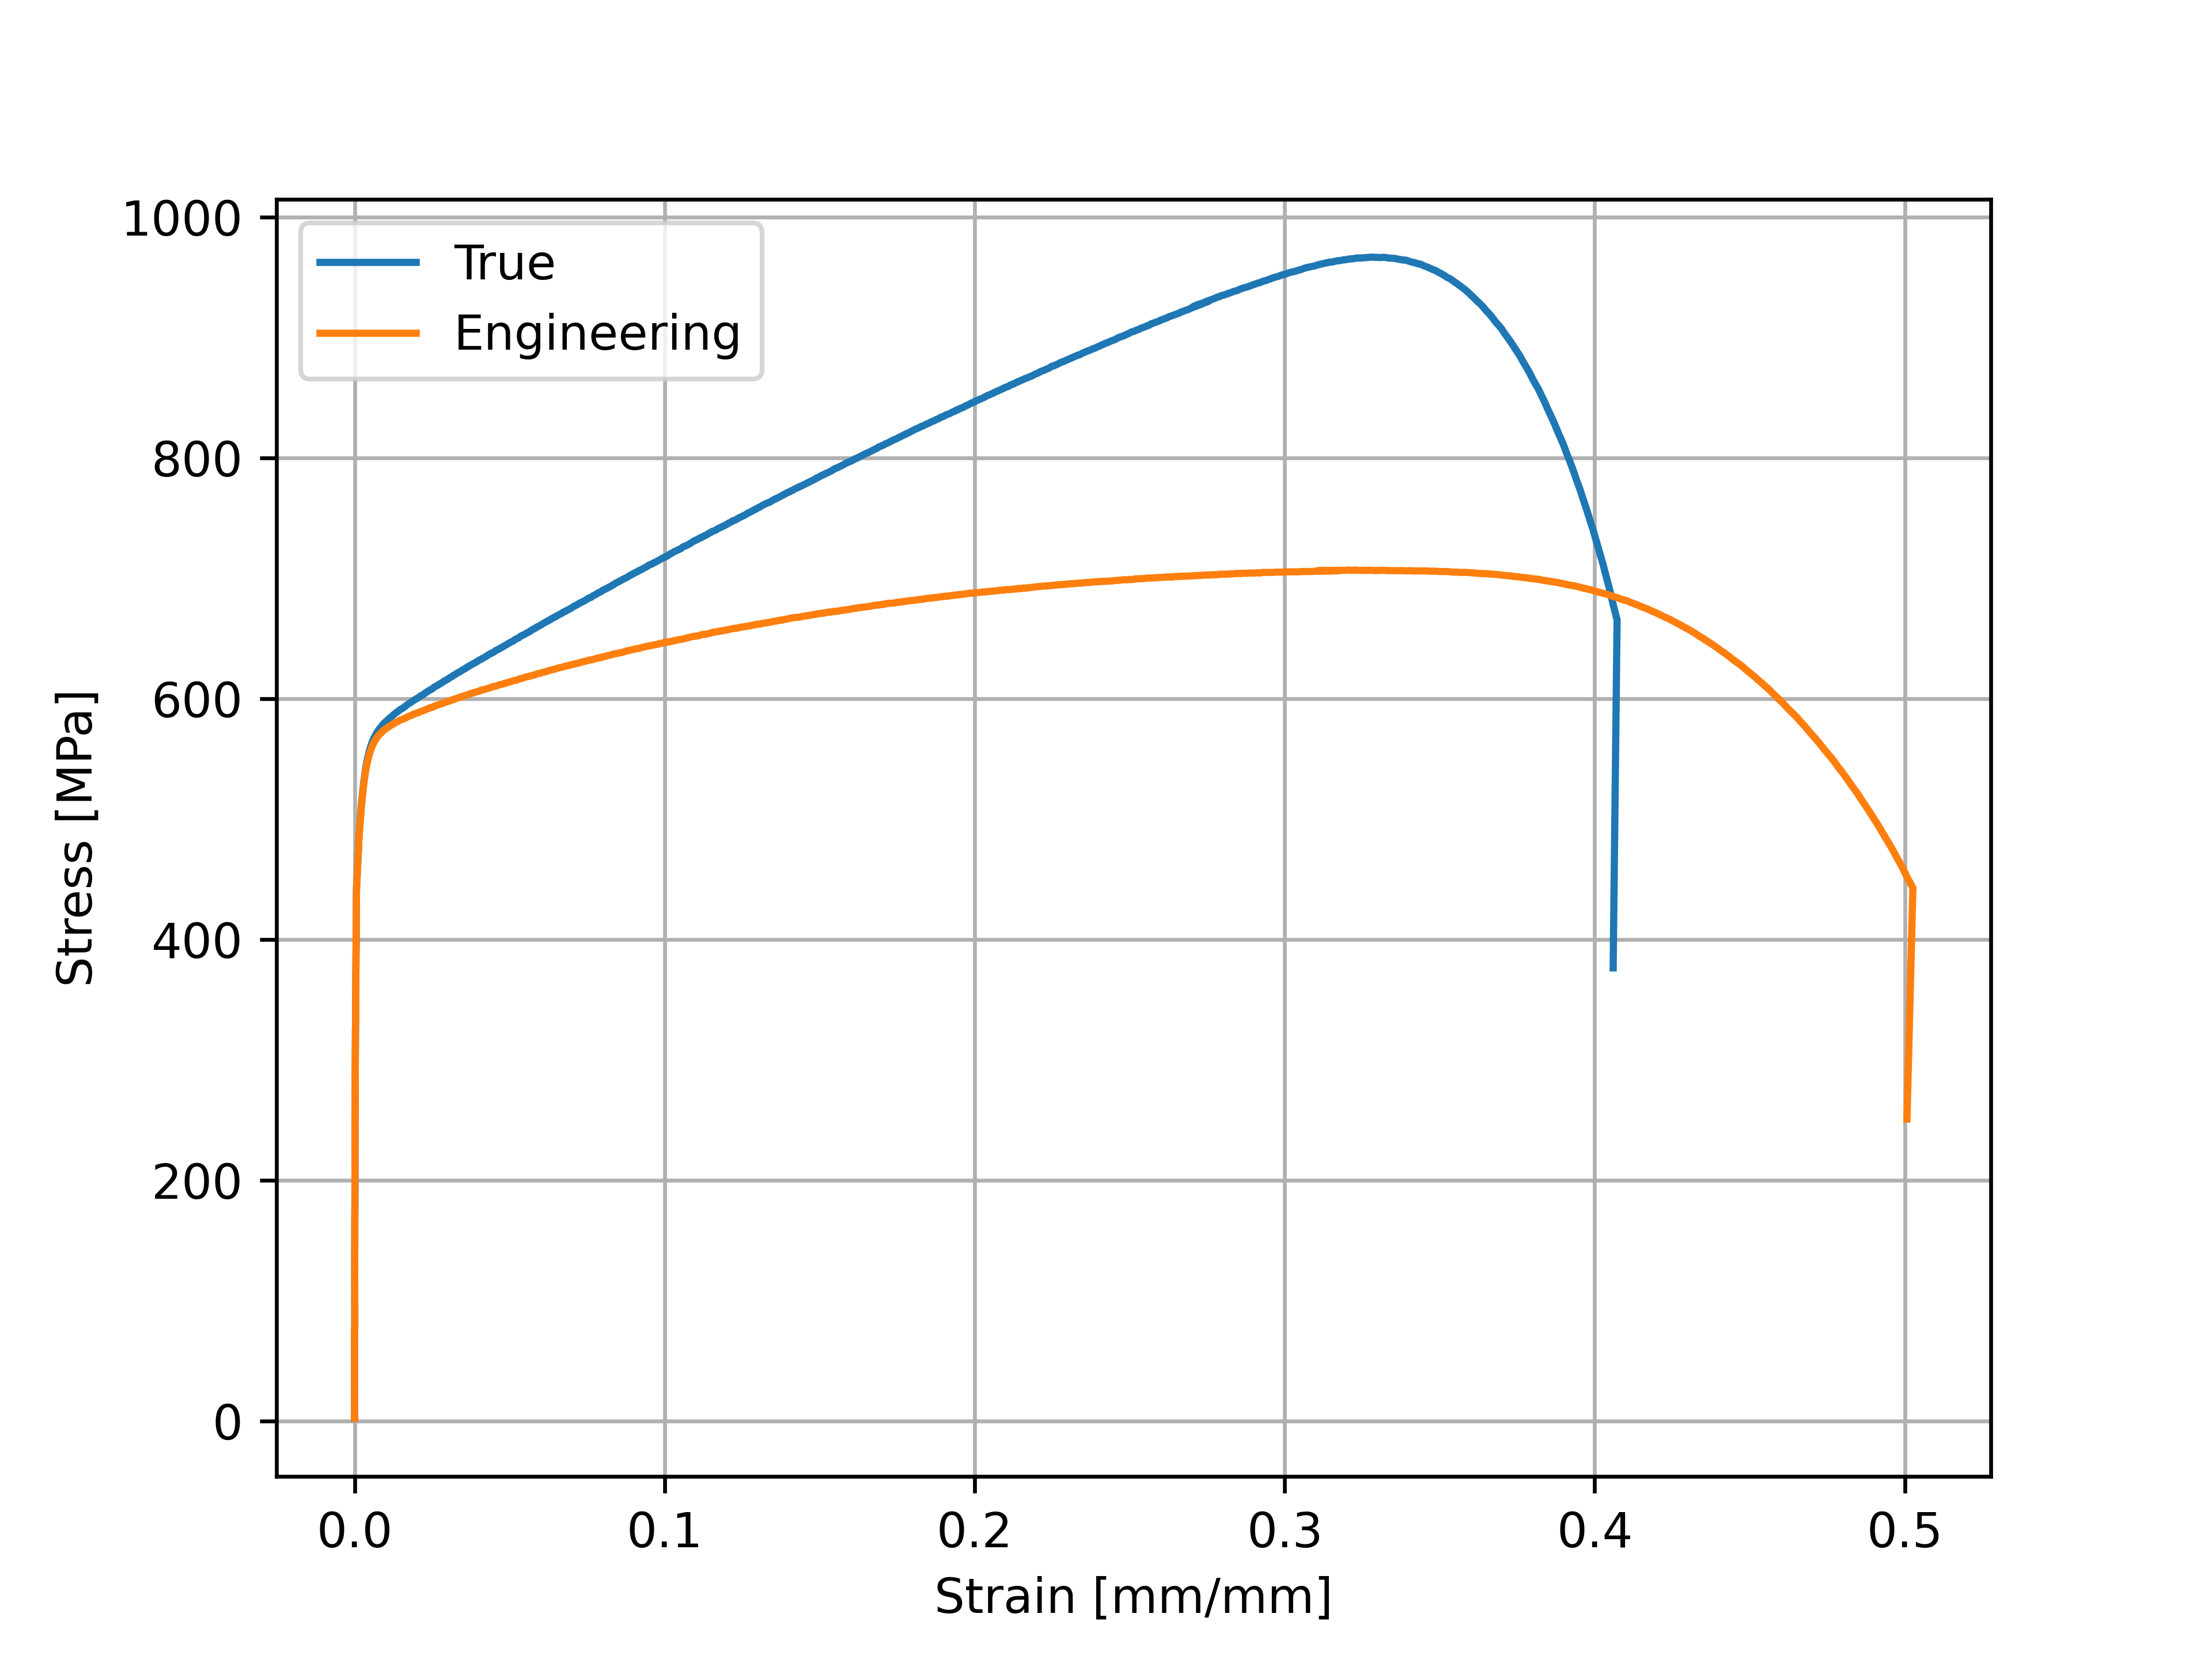
\includegraphics[width=0.5\linewidth]{plots/q4_evt.png}
    \caption{304 Stainless Steel engineering and true stress-strain}
    \label{fig:q4evt}
\end{figure}

\subsection{Question 5}
\begin{figure}[!h]
    \centering
    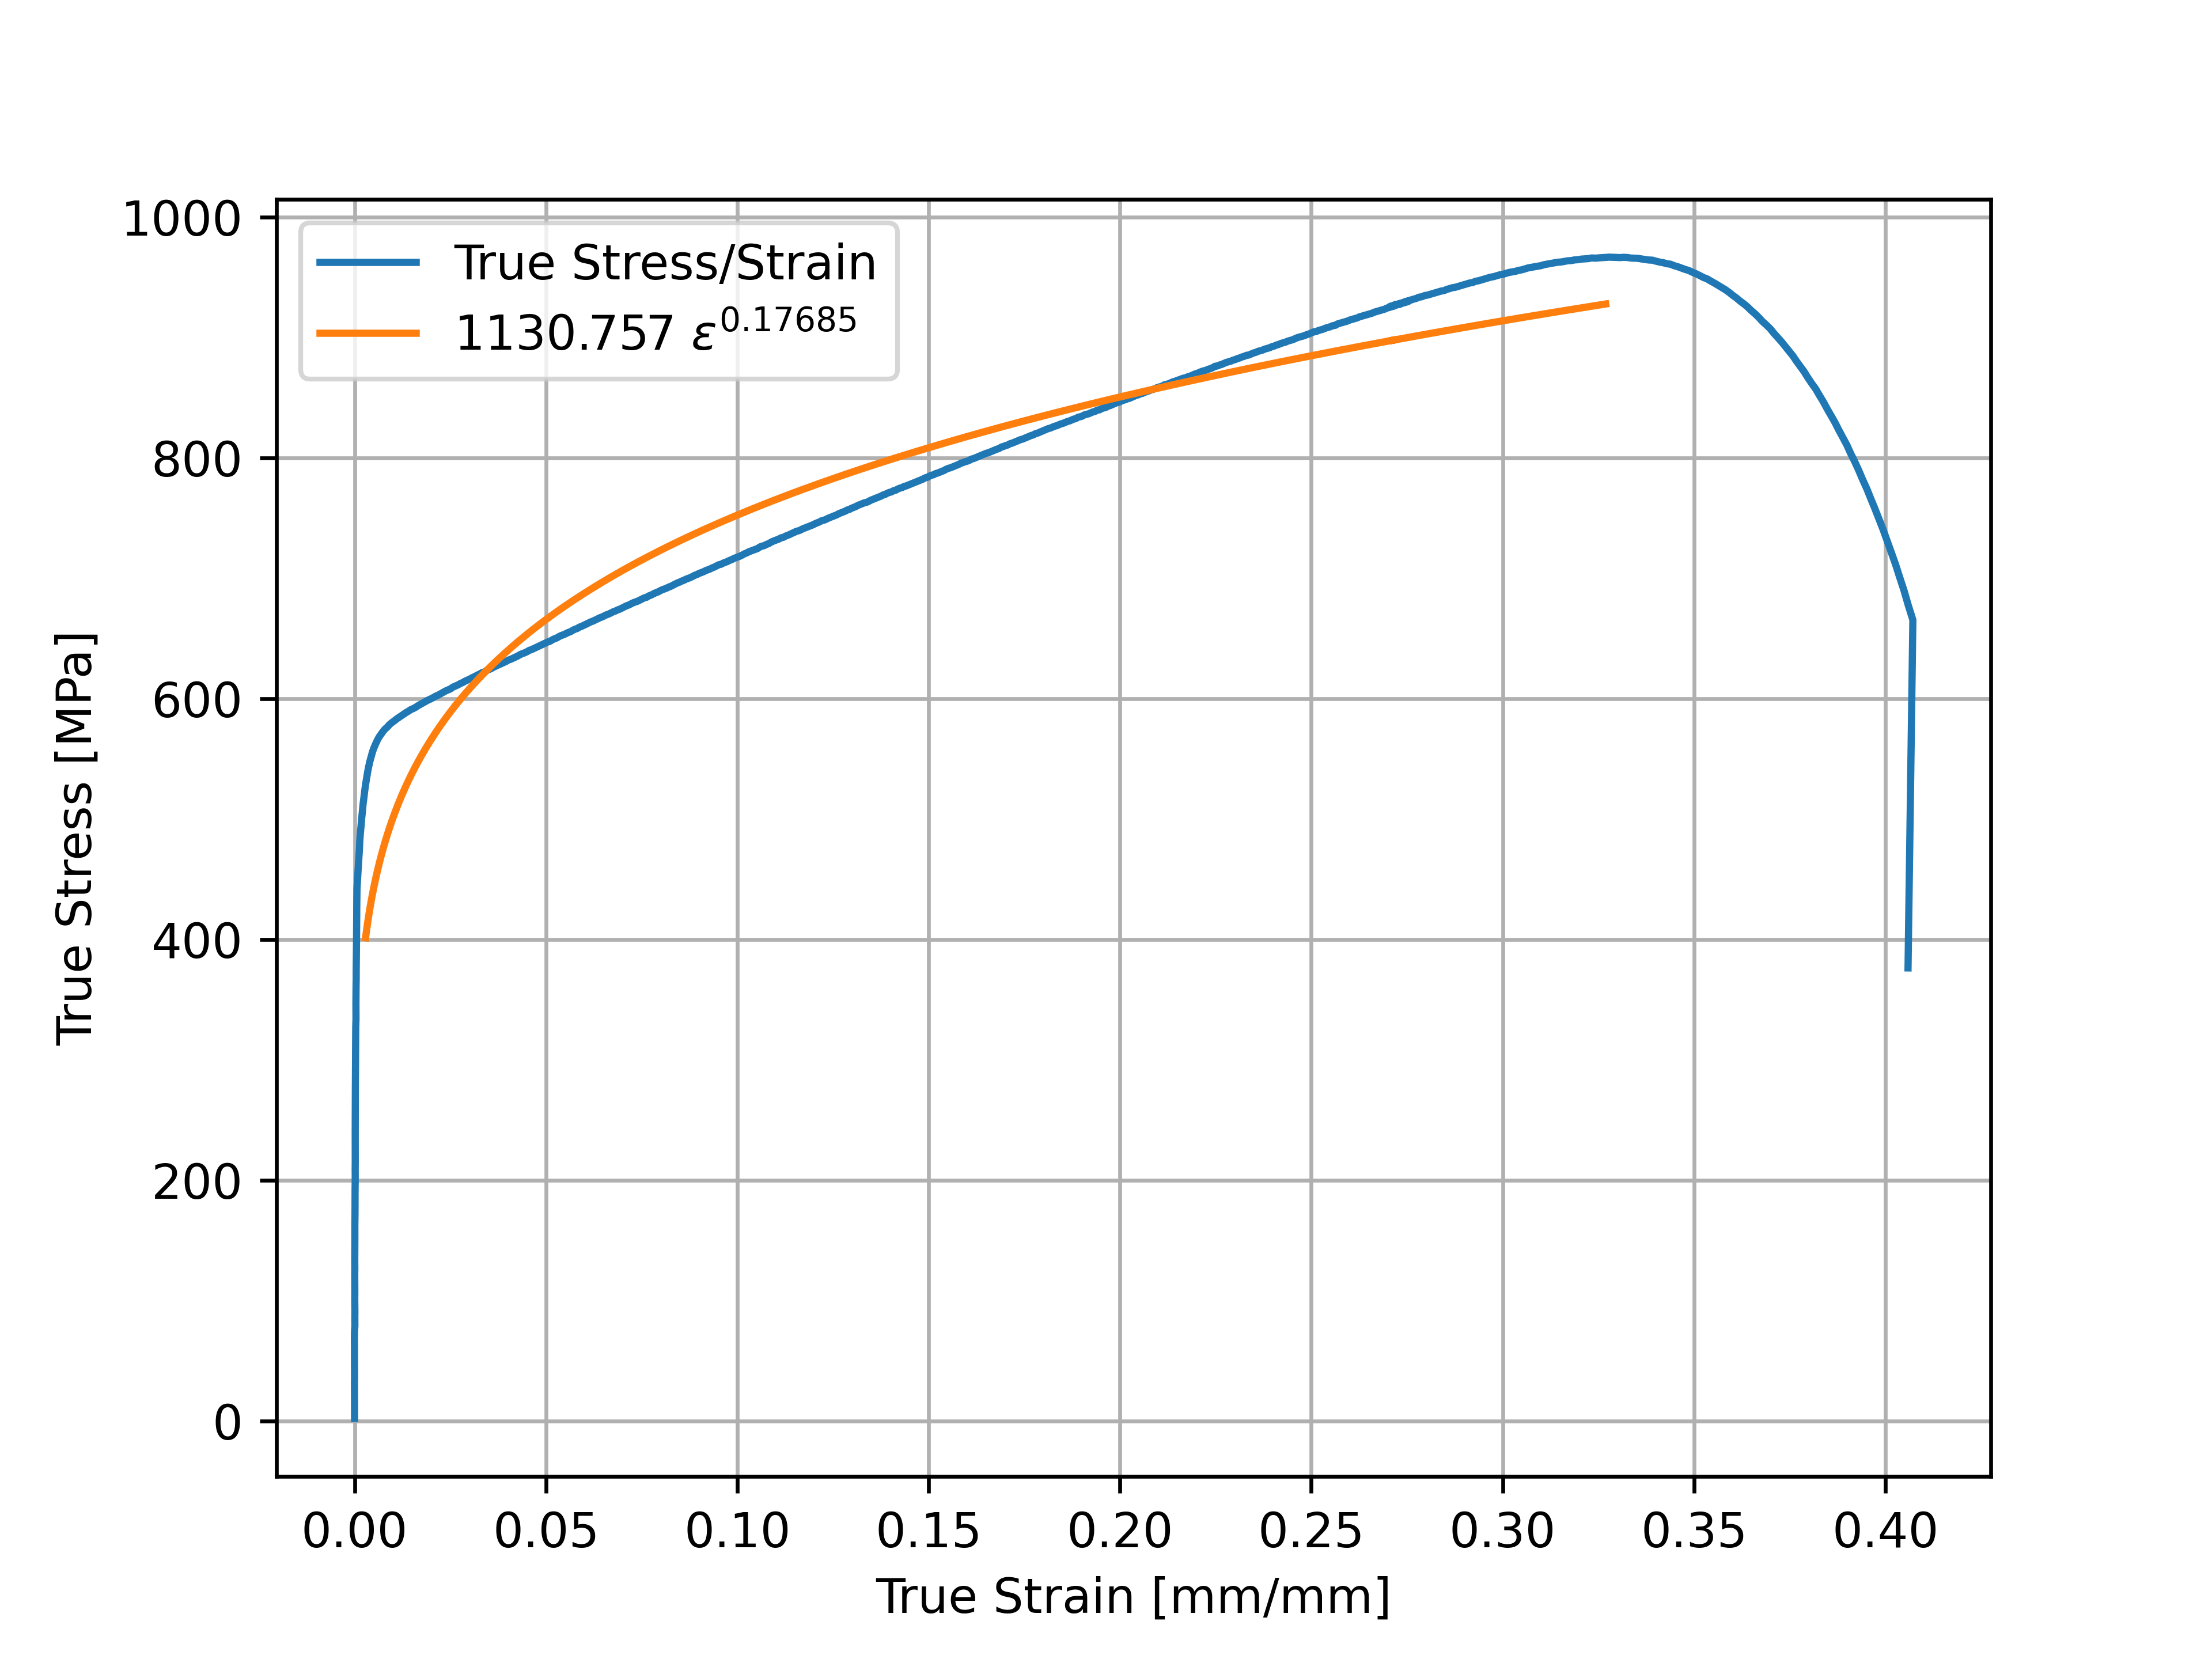
\includegraphics[width=0.5\linewidth]{plots/q5_fit.png}
    \caption{Power-Law fit of plastic deformation of 304 Stainless Steel}
    \label{fig:q5fit}
\end{figure}

\subsection{Question 6}
\begin{figure}[!h]
    \centering
    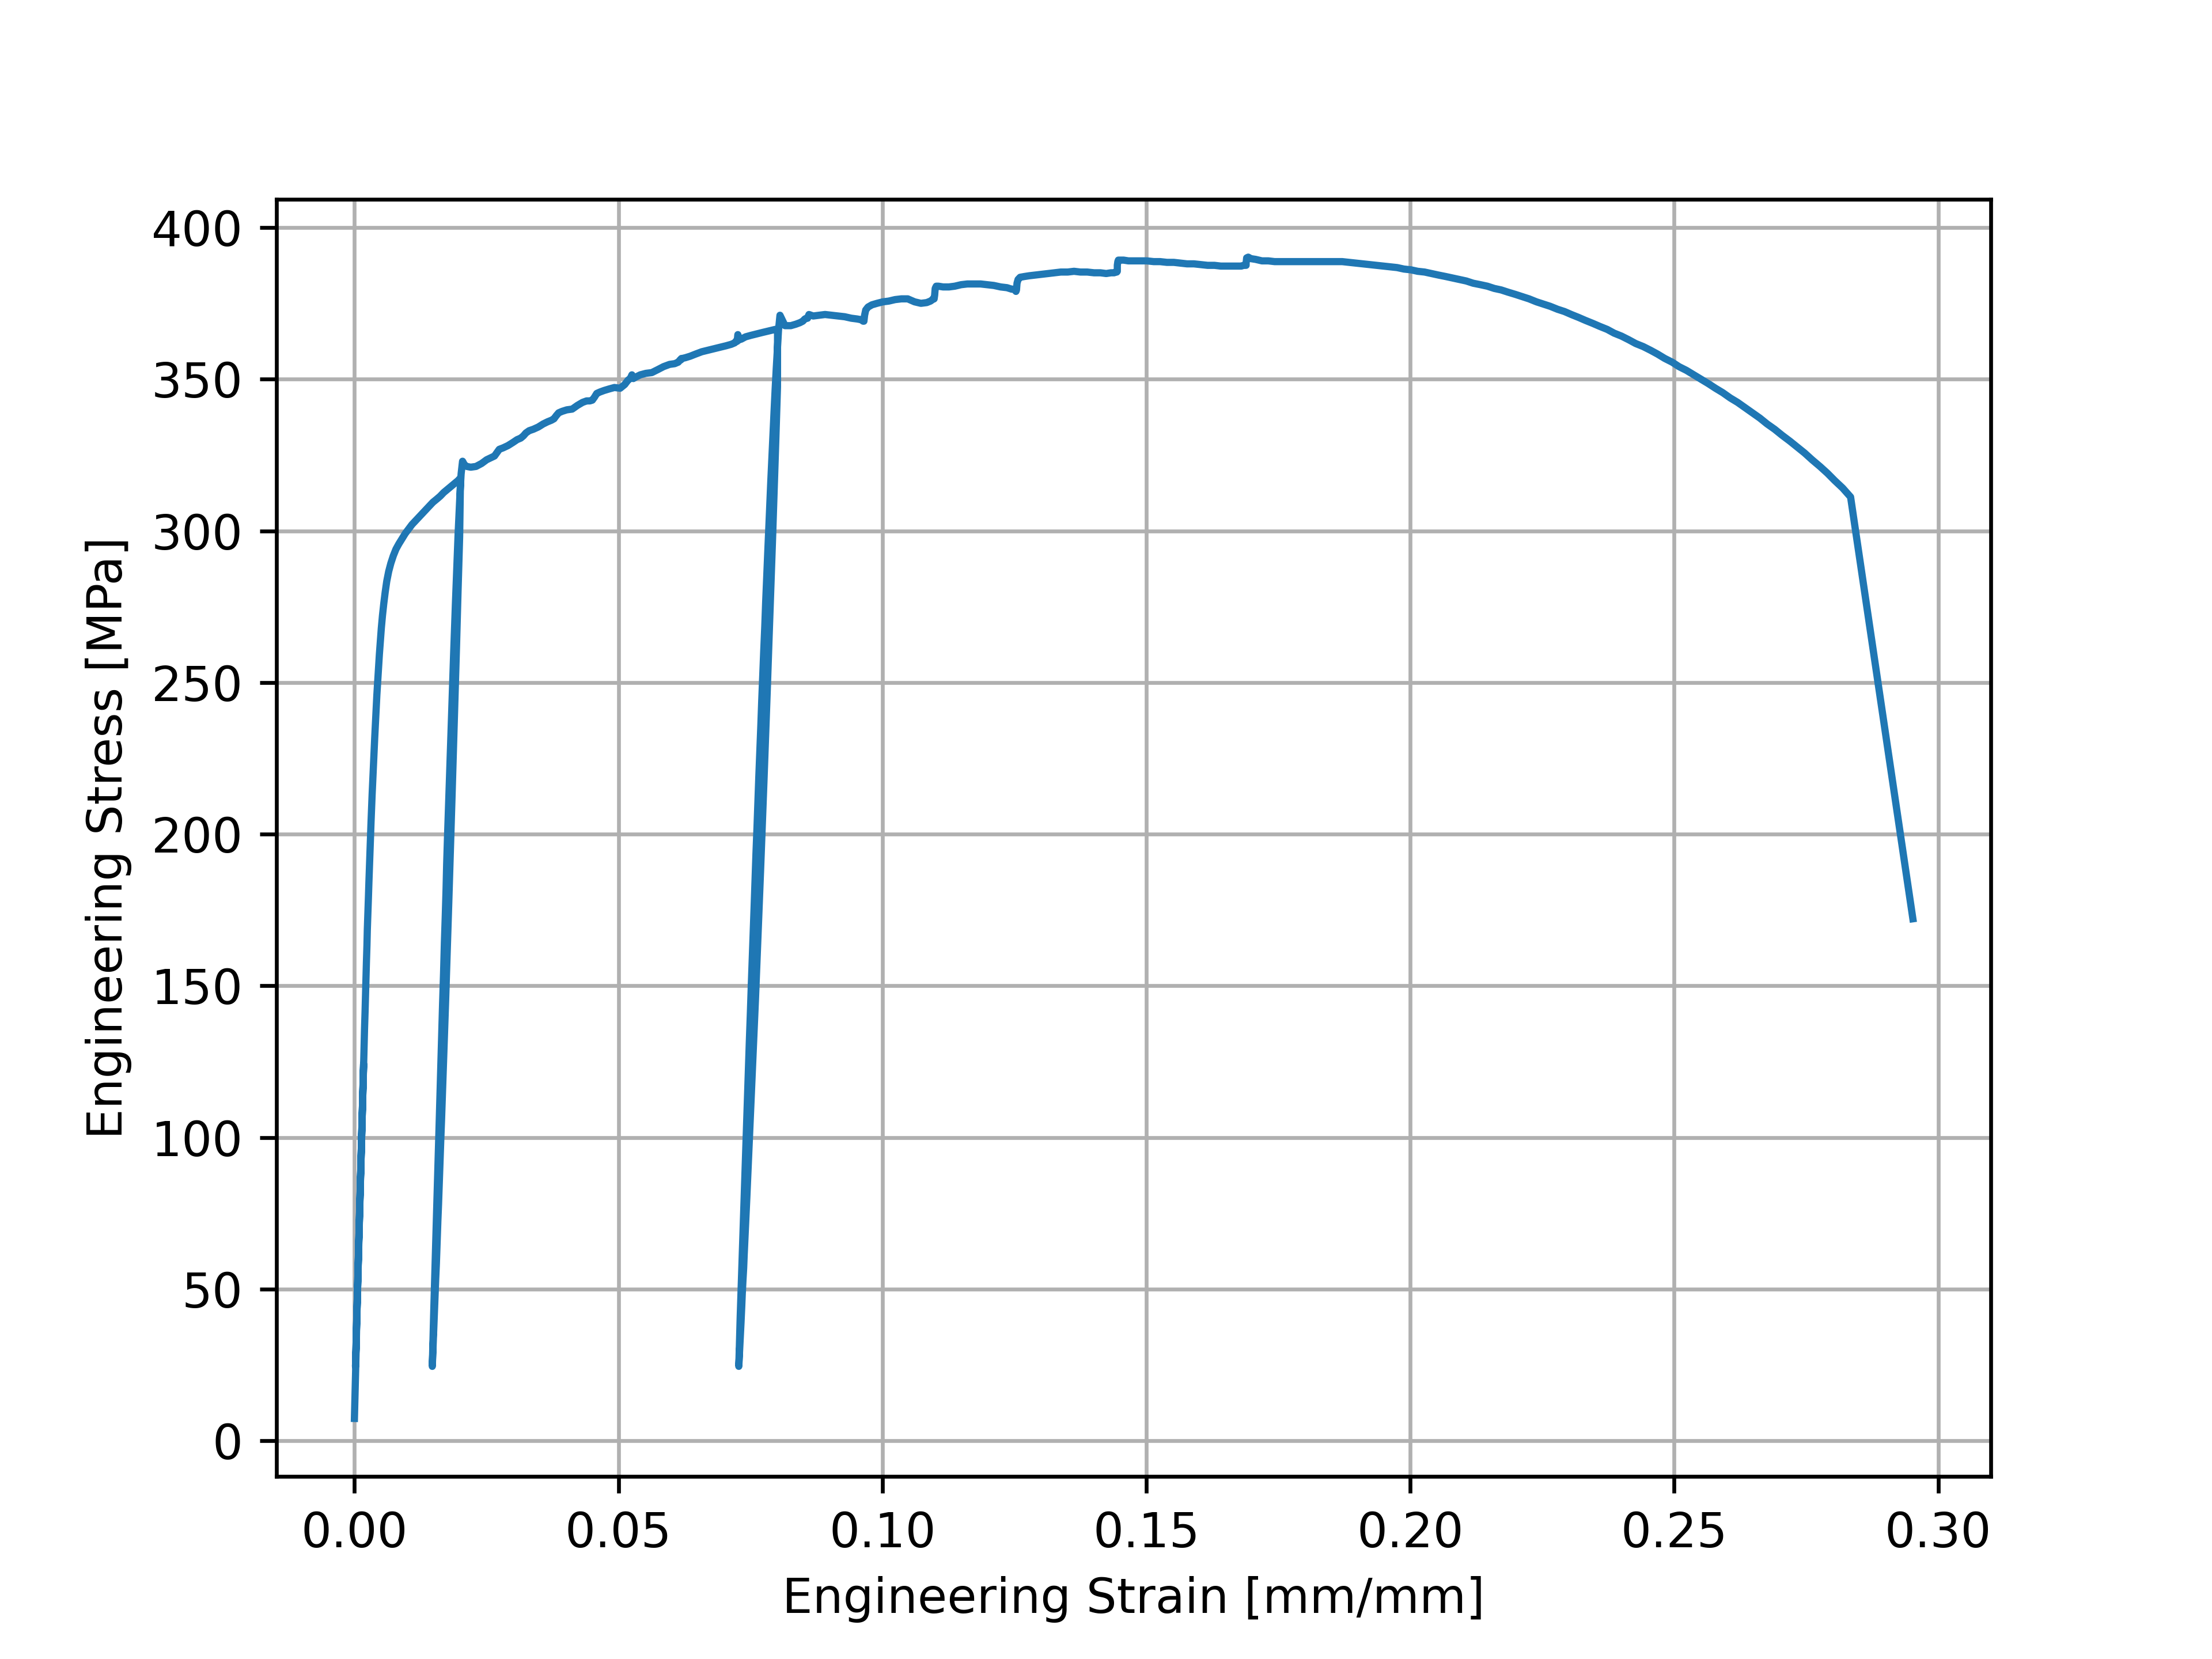
\includegraphics[width=0.5\linewidth]{plots/q6_br.png}
    \caption{Engineering stress-strain of cyclically loaded Bronze}
    \label{fig:br}
\end{figure}

\section{Analysis and Discussion}

\newpage
\section{Conclusions}
\newpage
\section{References}
\printbibliography[heading=none]

\end{document}